\documentclass{main}
 
 % New packages   
\usepackage[table,xcdraw]{xcolor}
%\usepackage{pdfpages}

%\usepackage[caption=false]{subfig}
       % required for bibliography
%\usepackage[brazilian]{babel}
%\newlength\shlength
%\captionsetup[subfigure]{labelformat=brace}

% --------------------------


\usepackage{graphicx}      % include this line if your document contains figures
\usepackage{natbib} 
\usepackage{enumerate}
\usepackage[utf8]{inputenc}
\usepackage{float}
\usepackage[centerlast,small,sc]{caption} 
\setlength{\captionmargin}{30pt}
\usepackage[none]{hyphenat} 
\usepackage{subcaption} 
\usepackage{capt-of}
\usepackage{kpfonts} 
\usepackage{calc}
\newcommand\xshlongvec[2][0]{\setlength\shlength{#1pt}%
  \stackengine{-5.6pt}{$#2$}{\smash{$\kern\shlength%
    \stackengine{7.55pt}{$\mathchar"017E$}%
      {\rule{\widthof{$#2$}}{.57pt}\kern.4pt}{O}{r}{F}{F}{L}\kern-\shlength$}}%
      {O}{c}{F}{T}{S}}
\sloppy      



\begin{document}

\begin{frontmatter}

%TODO Ajeitar o título para ser compatível com essa segunda fase.
\title{Estudo do conceito para metodologia e revestimento robótico
de turbinas \textit{in situ} - EMMA
\thanksref{footnoteinfo}} 

\thanks[footnoteinfo]{This work is supported by ESBR under contract COPPETEC
JIRAU 09/15 6631-0003/2015 (ANEEL R\&D program).}

\author[1]{Renan S. Freitas}
\author[1]{Gabriel Alcantara C. S.}
\author[1]{Eduardo Elael M. S.}
\author[1]{Estevão Fróes}
\author[1]{Ramon R. Costa}
%\author[2]{Sylvain Joyeux}
%\author[2]{Patrick M. Paranhos}

  \address[1]{Departamento de Engenharia Elétrica, COPPE UFRJ, Rio de Janeiro,
  Brasil} 
  % TODO Renan: Verificar departamento do patrick e sylvain
%  \address[2]{Centro de Inovação em Robótica (CIR), Rio de Janeiro, Brasil}
  
\begin{abstract}                % Abstract of not more than 250 words.
%TODO Renan: Resumo
\end{abstract} 
 
\begin{keyword}
%TODO Renan: Keywords
\end{keyword}

\end{frontmatter}

\section{Introdução}\label{sec::introducao}
%TODO Renan: Introdução
%TODO Situar o Leitor do que foi concluido no SOTA.

Em EMMA-SOTA, é apresentada a importância da manutenção regular das turbinas em
usinas hidrelétricas, já que, em sua operação ideal e de máxima eficiência, sua
potência tem aumento de quase 46\% após manutenção. Aumento significativo,
principalmente para países dependentes desta forma de energia, como o Brasil e
Noruega.

A eficiência de uma turbina hidrelétrica depende de inúmeras variáveis, como
volume de água, queda d'água, o tipo da turbina, o distribuidor e outras. O
projeto EMMA tem foco na manutenção do perfil hidráulico das pás dos rotores de
turbinas hidrelétricas, por este se degradar com maior rapidez, exigindo
manutenções recorrentes. A proteção da pá contra erosão é o processo de
revestimento por asperção térmica, ou, especificamente, a metalização (HVOF).
Atualmente, este processo pode levar cerca de dois meses por turbina, já que
exige que esta seja desmontada, cada pá processada em outro ambiente, a turbina
seja remontada e recalibrada.

Apesar de o projeto visar uma solução genérica para turbinas bulbo, as
instalações são diferentes em cada usina. Desta forma, o ambiente de testes
deste projeto é a Usina Hidrelétrica de Jirau, localizada no Rio Madeira e, portanto,
suas turbinas sofrem muito com erosão por cavitação e abrasão devido ao grande
número de partículas carregadas pelo rio e à baixa queda d'água. As principais
características das instalações da turbina em análise estão descritas em
EMMA-SOTA, mas vale ressaltar a peculiaridade dos dois acessos principais ao aro
câmara, relevantes para a busca de uma solução: acesso superior e acesso inferior.

O projeto EMMA busca uma solução para o processo de metalização \textit{in
situ}, isto é, revestimento das pás no ambiente da turbina, diminuindo o tempo
de manutenção e, consequentemente, de máquina parada.  A solução conceitual
desenvolvida é a utilização de um manipulador industrial sobre uma base. As
características do manipulador e da base variam de acordo com o ponto de acesso: no caso da escotilha superior, a solução é um
manipulador industrial de pequeno porte e base customizada operada
eletronicamente; no caso da escotilha inferior, a solução é um manipulador
industrial de porte médio e base tipo trilho com acopladores magnéticos.

A análise da Usina Hidrelétrica de Santo Antônio, em Porto Velho, vizinha à
Jirau, mostrou que as instalações da turbina não possuem a peculiaridade de um acesso
superior. A fim de tentar construir uma solução geral, o presente documento
visa dar continuidade ao projeto, detalhando o estudo de viabilidade técnica
para a solução da escotilha inferior.


%\section{Descrição do problema}\label{sec::consideracoes}

O fenômeno de cavitação e abrasão em hidroturbinas provoca desgaste
superficial por erosão e alteração do perfil
hidráulico da pá, gerando redução da eficiência na geração de energia.
Uma solução preventiva é o revestimento por metalização das pás, o qual aumenta a eficiência na
geração de energia por gerar uma estrutura mais lamelar, e fornecer maior
resistência a desgastes. No caso da usina hidrelétrica de Jirau, o revestimento
das pás é realizado antes da montagem e instalação da turbina, porém devido ao grande número de
partículas e sedimentos que o rio madeira carrega e à cavitação, o revestimento
deve ser aplicado novamente em intervalos curtos de tempo
\citep{santa2009slurry}. A desmontagem da turbina, aplicação de novo
revestimento nas pás e remontagem são um processo muito custoso e deverá ser
feito regularmente. Portanto, há a necessidade de o procedimento ser
executado dentro do aro câmara, \textit{in situ}, onde as pás são instaladas.

A cavitação é a formação de cavidades de vapor (bolhas), em um líquido, devido a
quedas repentinas de pressão. Quando o líquido é sujeito a aumento de pressão,
as bolhas implodem, ocasionando ondas de choque \citep{brennen2013cavitation}.

Em hidroturbinas, o fenômeno de cavitação é comum próximo às pás ou
na saída da turbina. O líquido apresenta combinação
de componentes cinético, potencial gravitacional e energia de fluxo. O
componente cinético é em virtude do fluxo da água (velocidade), a potencial tem
relação com a altitude, e a energia de fluxo é energia que um fluido contém
devido à pressão que possui. De acordo com o princípio de Bernoulli, o princípio
da conservação para os fluidos, implica-se que, para uma mesma altitude, o
aumento da componente cinética acarreta em uma diminuição da pressão, ocorrendo
cavitação. 

Quando há cavitação, a formação de bolhas grandes altera as características do
escoamento, ocasionando oscilações ou vibrações na máquina que, por
conseqüência, prejudicam o rendimento do sistema hidráulico. As bolhas
pequenas, ao colapsar, geram ondas de choque de alta frequência, podendo provocar erosões se
próximo à superfície metálica.

Além da cavitação, como a água atravessa o aro câmara em grande velocidade, o
acúmulo de sedimentos irá provocar desgaste abrasivo, isto é, perda de material
pela passagem dessas párticulas rígidas. 

Nesta seção, serão apresentadas as formas de reduzir os danos da cavitação pela
tecnologia de revestimento por metalização, a contextualização do problema no
caso da usina hidrelétrica de Jirau e as tarefas que um sistema robótico deve
realizar para solucionar o problema.


\subsection{Descrição do processo HVOF}\label{sec::desc_hvof}
O revestimento por aspersão térmica (ou metalização) é um processo em que
partículas aquecidas são pulverizadas em uma superfície a fim de melhorar ou
restaurar suas propriedades e dimensões. O revestimento estende a vida útil do
material, aumentando significantemente a sua resistência à erosão e corrosão.
Os diferentes tipos de metalização são: por chama, arco elétrico, detonação,
chama de alta velocidade (HVOF), plasma, a frio e a quente.

Um sistema de metalização é composto por: uma pistola de aspersão, responsável
pelo derretimento e aceleração das partículas a serem depositadas na
superfície; um alimentador, que fornece o pó (partículas) através de tubos;
um fornecedor do material de combustão; um robô para manipular a pistola; uma
fonte de alimentação elétrica para a pistola; um console de controle para o
sistema.

No caso específico das pás (aço inox 420) das turbinas da usina hidrelétrica de
Jirau, antes da montagem da turbina, a metalização tipo HVOF é realizada em
ambos os lados da pá pela empresa Rijeza com um manipulador industrial de 150 kg
de carga máxima, permitindo controle de vibrações com boa margem de segurança, já que a massa do
sistema pode chegar a 20 kg (cabos e pistola). O tempo
médio do processo é de 6 horas por lado da pá.

Primeiramente, a pá é preparada por jateamento com óxido de alumínio. O HVOF
consiste em alimentar, numa câmara de combustão, o material de revestimento
(carboneto de tungstênio) e uma mistura gasosa do combustível (propano) e
oxigênio. De acordo com os dados fornecidos pela empresa Rijeza, a pistola de 8
Kg projeta uma chama de $3000^oC$, que pulveriza as partículas com velocidade de
700 a 1000 m/s, gerando uma força de recuo de 15 N.

O manipulador robótico deve possuir precisão de 5 mm, a pistola no efetuador
deve permanecer a uma distância que varia entre 230 e 240 mm, e ângulo de $30^0$
a $90^0$, em relação à superfície. O manipulador deve ser capaz de mover a
pistola a velocidade constante de 40 m/min, e não pode estar fixa em uma posição
da pá por muito tempo (parada), pois há acúmulo de material, deformando a
superfície. Trocas de direção ou sentido na movimentação do manipulador são
considerados como parada, logo as trocas deverão ser realizadas em áreas
exteriores à superfície da pá ou chapas de sacrifício são utilizadas. 

Placas de sacrifício, ou mascaramento, são chapas colocadas em regões onde as
peça não podem ser jateadas ou revestidas. Geralmente uma chapa de qualquer tipo
de aço pode ser utilizada, pois a chama não fica parada sobre ela por um longo
período, não aquecendo-a o suficiente para danificar. Quando a pistola fica
parada, em funcionamento, a chama é apontada para algum lugar onde não tenha
obstáculos.

 % As informações do processo
% podem ser observadas na figura~\ref{fig::hvof}.
 
%\begin{figure}[h!]	
%	\includegraphics[width=\columnwidth]{figs/intro/hvof.pdf}
%	\caption{Foto do efetuador do manipulador e pistola HVOF.}
%	\label{fig::hvof}
%\end{figure}

Em relação às condições de operação, o espaço da aplicação HVOF é confinado, com
excesso de ruído de 100 a 140 dB, gases nocivos e com risco de explosão podem
ser exalados, a pá pode atingir temperaturas de até $110^oC$, as condições de
umidade e temperatura devem ser ideais para o processo e há perda de $40\%$
das partículas pulverizadas  \citep{wu2006rebound}, que são espalhadas pelo
ambiente. Portanto, a operação deve ser remota, não há presença de pessoas \textit{in loco}, os gases
presentes e umidade/temperatura devem ser constantemente monitorados, o robô
manipulador é selado e as partículas desperdiçadas devem ser removidas
(limpeza). Como forma de segurança contra gases explosivos, o desligamento do
sistema é imediato por corte de gás, porém, em caso de falta de energia, o
manipulador será desligado, mas a chama não se apagará.

A qualidade do revestimento é geralmente avaliada por um instrumento que
realiza a medida de porosidade, oxidação, dureza e rugosidade da superfície. O
processo é realizado manualmente, de maneira rápida e fácil, por um operador e
pontos específicos da pá são analisados.

A tabela~\ref{tab::hvof} resume as restrições e especificações do
projeto:

\begin{center}
\begin{tabular}{  c | c  }
  \hline
  \textbf{Componente} & \textbf{Dado} \\ \hline
  Massa da pistola HVOF & 8 Kg  \\ \hline
  Massa dos cabos HVOF & 12 Kg  \\ \hline
  Tempo HVOF por pá & 6 horas \\ \hline
  Temperatura da chama HVOF & $3000^oC$ \\ \hline
  Recuo da pistola & 15 N \\ \hline
  Precisão do manipulador & 5 mm \\ \hline
  Distância pistola-pá & 230-240 mm \\ \hline
  Ângulo pistola-pá & $30^o$-$90^o$ \\ \hline
  Velocidade do manipulador & 40 m/s \\ \hline
  Ruído HVOF & 100 a 140 dB \\ \hline
  Temperatura da pá & $110^oC$ \\
  \hline
\end{tabular}
\captionof{table}{Dados principais do processo HVOF}
%\caption{Dados principais do processo de metalização HVOF}
\label{tab::hvof}
\end{center}

%Sistemas robóticos não devem utilizar magnetismo como meio de aderência, já que
%o aço inox 420 não apresenta alta permeabilidade magnética e a alta temperatura
%da pá deve inviabilizar essa solução. Adesão por ventosas é uma solução
%viável, pois material não causa dano ao revestimento, porém a escolha do
%material da ventosa deve ser estudado,já que a pá quente pode ocasionar em
%perda de sucção, como em ventosas emborrachadas.


\subsection{Contextualização do Ambiente}\label{sec::desc_contex}

A usina hidrelétrica de Jirau é do tipo fio d'água, na qual são utilizadas turbinas do tipo bulbo de eixo horizontal. Como a geração de energia depende da altura da queda
d'água e da vazão do rio, as turbinas do tipo bulbo utilizam uma grande vazão de
água para produzirem energia elétrica suficiente. A figura
\ref{fig::bulb_turbine} e a tabela \ref{tab::bulb_turbine} ilustram uma turbina
do tipo bulbo e o grandes dutos necessários para comportar o grande volume de água que passa através da turbina. 
 
\begin{figure}[h!]	
	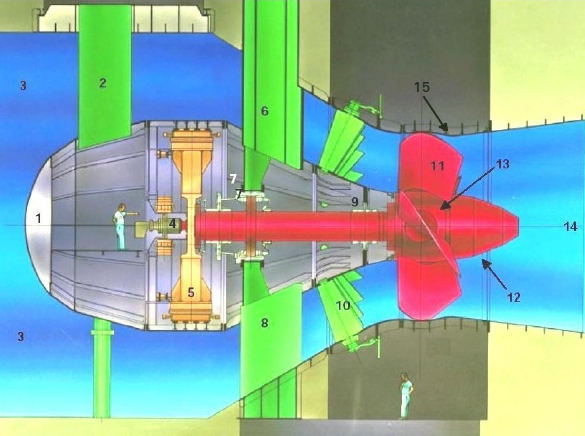
\includegraphics[width=\columnwidth]{figs/intro/bulb_turbine2}
	\caption{Ilustração de uma turbina do tipo bulbo.}
	\label{fig::bulb_turbine}
\end{figure}

\begin{center}
\begin{tabular}{  c | c  }
  \hline
  \textbf{Número} & \textbf{Componente} \\ \hline
  1 & Nariz do bulbo \\ \hline
  2 & Tubo de acesso ao gerador  \\ \hline
  3 & Câmara de adução  \\ \hline
  4 & Cabeçote Kaplan  \\ \hline
  5 & Gerador Síncrono  \\ \hline
  6 e 8 & Estrutura de sustentação \\ \hline
  6 & Tubo de acesso à turbina \\ \hline
  7 e 9 & Mancais Combinado e Guia \\ \hline
  10 & Distribuidor \\ \hline
  11 & Pás do Rotor \\ \hline
  12 & Cone ou Ogiva \\ \hline
  13 & Cubo \\ \hline
  14 & Tubo de sucção/descarga \\ \hline
  15 & Aro Câmara \\
  \hline
\end{tabular}
\captionof{table}{Componentes principais de uma turbina tipo bulbo}
%\caption{Componentes principais de uma turbina tipo bulbo}
\label{tab::bulb_turbine}
\end{center}



Atualmente, caso seja necessário algum reparo ou inspeção na turbina, é necessário que se interrompa o fluxo de água e que 
toda a água em seu interior seja drenada. Para manutenção do rotor, existe uma escotilha de acesso de diâmetro limitado. Entretanto, caso deseje-se realizar 
a metalização de pás já instaladas, utilizando-se os processos atuais, é
necessária a retirada de todo o aro câmara, desmontagem completa do rotor e logística de transporte das pás até o local
onde a metalização será realizada. Essa operação, caso necessite ser realizada, demandaria a mobilização
de diversas equipes de manutenção, operação de pórtico rolante e transporte,
além de impossibilitar a utilização da turbina durante várias semanas.
No contexto da solução proposta, os pontos de interesse da turbina são:

\begin{itemize}
  \item Hélice e pás;
  \item Aro Câmara e regiões adjacentes;
  \item Escotilhas de acesso;
  \item Tubo de Sucção;
  \item Infraestrutura disponível
\end{itemize} 

\subsubsection{Hélice e pás}
 
O rotor ou hélice da turbina é constituído, basicamente, do cubo, as pás e o cone. 
Nas turbinas da usina de Jirau, cada pá mede, aproximadamente, 2,5m de altura e
3m de largura. A partir do interior da turbina, todas as superfícies da pá são
alcançáveis, com exceção da borda e do lip da pá. O único ponto de acesso à
essa regiâo é por meio da escotilha superior de acesso. A figura
\ref{fig::blade_rijeza} exemplifica uma pá do rotor presente na usina de Jirau recém metalizada no galpão da Rijeza.

\begin{figure}[h!]	
	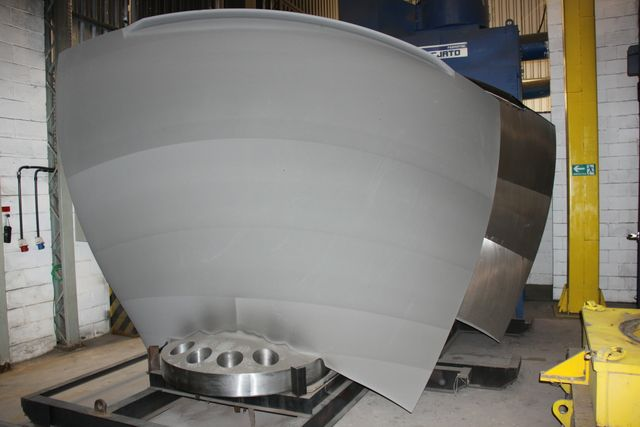
\includegraphics[width=\columnwidth]{figs/viagem/2015_04_28/Rijeza/img_4887}
	\caption{Pá do rotor recém metalizada.}
	\label{fig::blade_rijeza}
\end{figure}

A agulação de cada pá em relação ao fluxo d'água pode ser alterado em 29$^o$, 14,5$^o$ para cada 
lado a partir da posição inicial, não havendo sobreposição entre as pás, como
ilustrado na figura \ref{fig::blades_angle}.
Essa angulação pode ser explorada para otimizar o espaço de trabalho necessário
para o processamento da pá e também influencia o acesso à região
entre o distribuidor e o rotor, uma vez que não existe acesso pela montante da turbina. A posição do 
rotor também pode ser manualmente alterada, possibilitando 
que o mesmo seja girado em ambas as direções e sem limite de revoluções. Entretanto, essa operação 
é uma tarefa complicada e envolve um certo risco às pessoas que a realizam. Sendo assim, a solução 
proposta deve otimizar o número de rotações necessárias para o processamento de todas as pás.

\begin{figure}[h!]	
	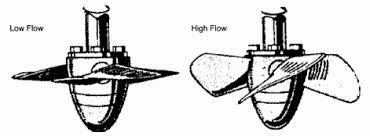
\includegraphics[width=\columnwidth]{figs/intro/blades_angle}
	\caption{Exemplo de limites de rotação das pás do rotor.}
	\label{fig::blades_angle}
\end{figure}

Na usina de Jirau, foram verificados a presença do fenômenos de abrasão e cavitação. O primeiro é 
causado principalmente pelo grande número de partículas e detritos presentes no Rio Madeira. Por 
sua vez, o fenômeno de cavitação é tem sua presença intensificada, segundo estudos realizados na 
própria usina, para quedas com mais de 12 metros de diferença. Foi observado também danos em ambos 
os lados da pá, ou seja, em Jirau há presença de cavitação por fenômenos de alta e baixa pressão. 

A manutenção dos danos causados, assim como a metalização preventiva, é diferenciada para abrasão 
e cavitação. O processo de metalização utiliza diferentes ligas para cada tipo de fenômeno e é 
imporante que não haja concomitância de ambos os processos em alguma região da pá. O desgaste de 
material devido a cavitação deve ser compensado por meio da deposição de material utilizando-se solda. 
O processo de metalização não é capaz de depositar a quantidade de material necessária e também não 
possui a precisão necessária para preencher somente as regiões afetadas. 

A deposição de solda nos orifícios causados pela cavitação deve ser feito de maneira controlada 
para que não haja alteração do perfil hidráulico da pá. Entretanto, o modelo exato do perfil da 
pá não é fornecido pelo fabricante e deverá ser construído em uma pá modelo para que seja possível 
a reparação desses danos.


\subsubsection{Aro Câmara e regiões adjacentes}

O aro câmara, assim como o a região próxima ao distribuidor e também ao tubo de
sucção são superfícies metálicas. Essa característica possibilita a exploração de soluções de fixação magnética.

Somente a região compreendida pelo aro câmara é plana e tendo como agravante a presença do distribuidor na região à 
montante ao rotor. É necessário que a inclinação presente nessas superfícies seja contabilizada e uma solução eficiente 
de apoio ou plano elevado seja desenvolvida caso haja necessidade de fixação de alguma parte do sistema. Atualmente todo 
o trabalho é realizado por meio da montagem de andaimes ancorados por cordas. A
figura \ref{fig::andaime} ilustra uma estrutura utilizada no modo de inspeção e
manutenção atuais.

\begin{figure}[h!]	
	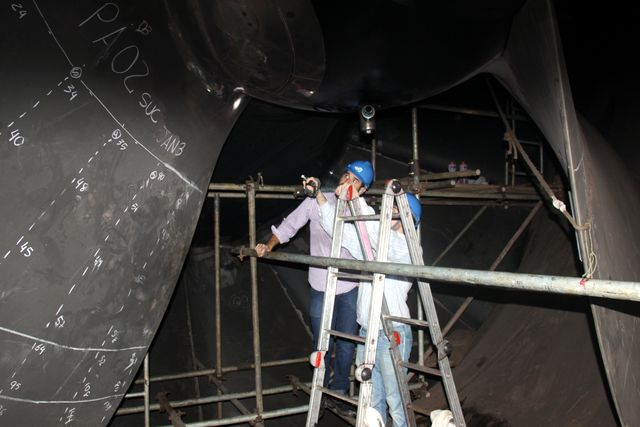
\includegraphics[width=\columnwidth]{figs/viagem/2015_04_28/UG/img_4969}
	\caption{Andaime montado no interior da turbina e ancorado por cordas}
	\label{fig::andaime}
\end{figure}

 
\subsubsection{Escotilhas de acesso}
O acesso à turbina se dá por duas escotilhas, uma inferior, localizada no ínicio do tubo de sucção 
próxima ao aro câmara e outra superior, localizada na parte superior do aro câmara.

A escotilha inferior é o acesso utilizado para a entrada de pessoas na turbina e, atualmente, todo 
material utilizado para reparos é transportado através dessa escotilha. Na usina de Jirau existem dois 
tipos de escotilha de acesso inferior, sendo a menor delas possuindo 80cm de diâmetro. 

A escotilha superior é utilizada, principalmente, para a inspeção visual do estado do Lip. 
O diâmetro do acesso superior é de aproximadamente 45cm, limitando as dimensões dos equipamentos que podem 
ser transportados através da escotilha. As figuras \ref{fig::esc_sup_ext} e
\ref{fig::esc_sup_int} ilustram o acesso à escotilha superior pelo exterior ao
aro câmara e também a visão da escotilha pelo interior da turbina,
respectivamente.

\begin{figure}[h!]	
	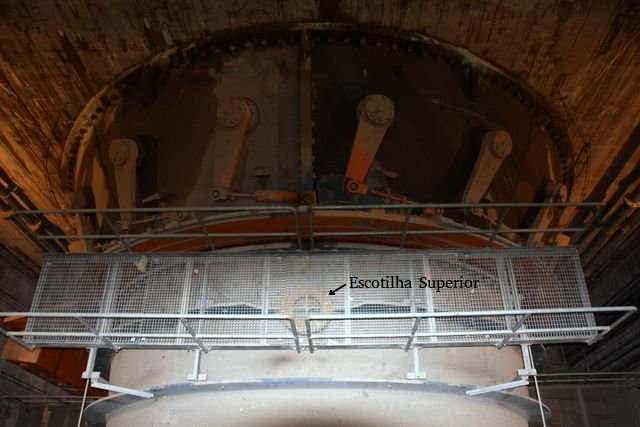
\includegraphics[width=\columnwidth]{figs/viagem/2015_04_28/UG/img_4979_mod}
	\caption{Vista da escotilha superior pelo exterior do aro câmara}
	\label{fig::esc_sup_ext}
\end{figure}

\begin{figure}[h!]	
	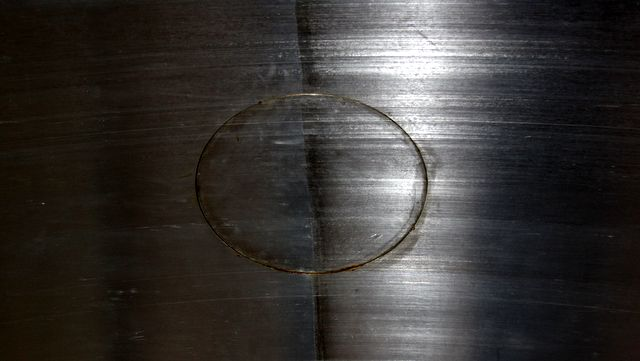
\includegraphics[width=\columnwidth]{figs/viagem/2015_04_28/UG/img_4982}
	\caption{Vista da escotilha superior pelo interior do aro câmara}
	\label{fig::esc_sup_int}
\end{figure}

\subsubsection{Tubo de sucção}

O tubo de sucção é relevante ao contexto dessa proposta pois caracteriza uma 
possibilidade de acesso. Ao final do tubo de descarga está localizado o vão dos stoplogs 
de jusante ou da comporta vagão e, em seguida, o leito do rio. Caso os stoplogs 
não estejam inseridos, existe um vão de acesso de pelo menos 10m de largura. O 
fluxo de água pode ser controlado pela abertura do distribuidor, criando assim 
um acesso extra para um sistema submarino. A figura \ref{fig::tubo_suc}
exemplifica a magnitude do tamanho do acesso, deixando claro que o limitante de
tamanho do sistema para a utilização desse acesso é o vão de entrada do stoplog,
ilustrado na figura \ref{fig::stoplog}. Outra alternativa é utilizar um
guindaste e submergir o sistema pelo próprio rio, entretanto o sistema ficaria
sujeito as condições do ambiente.

\begin{figure}[H]	
	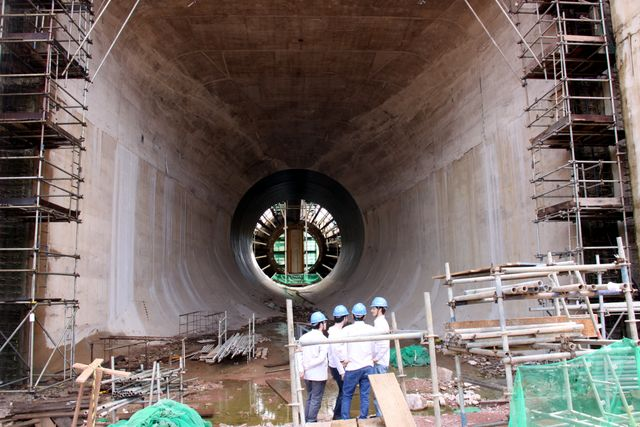
\includegraphics[width=\columnwidth]{figs/viagem/2015_04_30/Vao/img_5086}
	\caption{Abertura do tubo de sucção para o leito do rio, em fase de
	construção.}
	\label{fig::tubo_suc}
\end{figure}

\subsubsection{Infraestrutura disponível}
É importante ressaltar a infraestrutura dísponível para o desenvolvimento da solução. 
Após seca a turbina, é possível a disponibilização de energia elétrica e ar comprimo 
em seu interior, ambos importantes para o processo de metalização. Outro fator 
importante é a presença de um pórtico rolante que tem acesso até o andar diretamente 
inferior ao aro câmara, posicionando todo o equipamento necessário nas proximidades 
da escotilha de acesso inferior. É possível também o acesso direto, por meio de pórtico, 
à escotilha superior.

\begin{figure}[h!]	
	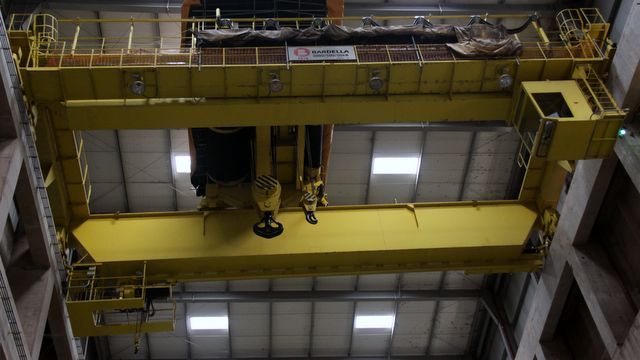
\includegraphics[width=\columnwidth]{figs/viagem/2015_04_28/UG/img_4989}
	\caption{Pórtico rolante com acesso ao exterior do aro câmara}
	\label{fig::portico}
\end{figure}


O ambiente pode ser resumidamente caracterizado pelas dimensões das pás,
elemento a ser processado; características do aro câmara, estrutura que limita o
espaço de trabalho do robô; e pelos acessos nos quais o sistema terá que
utilizar.

\begin{itemize}
  \item \textbf{Pás do rotor} - Material aço inox 420. Dimensões 2.5 x 2.5 m de superfície;
  \item \textbf{Aro Câmara} - estrutura cilíndrica com raio de 3.95 m e
  superfície metálica;
  \item \textbf{Acessos}: 
  	\begin{itemize}
    	\item Escotilha superior - 35 cm de diâmetro;
  		\item Escotilha inferior - 80 cm de diâmetro;
  		\item Tubo de descarga - 20 x 20 m, porém acessado pelo rio. 
  	\end{itemize}
\end{itemize}










\section{Estudo de viabilidade técnica detalhada}\label{sec::viatec} 
% Author: Renan

O estudo de viabilidade técnica detalhada é realizado para cada acesso à turbina
(superior e inferior), como em EMMA-SOTA. O estudo passa pelas
seguintes etapas: 1) pesquisa de mercado; 2) geometria plana e/ou espacial; 3)
espaço de trabalho e cinemática do manipulador; 4) detalhamento de
bases mecânicas; 5) dinâmica do manipulador; 6) sensores para calibração; 7)
planejamento de trajetórias; e 8) técnicas de calibração.
Neste documento, serão abordadas as etapas: 1, 2, 3, 4, 5 e 6.

A pesquisa de mercado é uma busca abrangente de soluções comerciais dentro do
escopo da solução conceitual desenvolvida no EMMA-SOTA. A pesquisa envolve
manipuladores comerciais que preencham os requisitos do processo de HVOF e
estejam de acordo com as restrições impostas pelo ambiente e o acesso. Desssa
forma, diversos fabricantes de manipuladores, Motoman, Kuka, ABB, Fanuc,
Adept e Kinova, foram avaliados e suas principais características como carga,
peso, dimensões, velocidade, temperatura e umidade de operação, são analisadas.
A pesquisa de mercado tem como objetivo retornar o objeto para os outros
estudos, ou seja, o manipulador a ser utilizado na solução.

O estudo puramente geométrico, apesar de ser diferente para cada acesso, é
genericamente uma abordagem simplificada e analítica do problema e desconsidera
alguns fatores do ambiente. O estudo geométrico tem como objetivo retornar um caso
aproximado da situação real e estimar as possíveis soluções da posição do
manipulador em relação à pá, de forma que toda ela seja revestida.

O espaço de trabalho e cinemática do manipulador é uma abordagem
detalhada e de simulação. Ela considera: o meio estruturado, em um ambiente de
simulação; o manipulador com suas dimensões e limites de juntas reais;
possibilidade de colisões; real espaço de trabalho do manipulador; modelos de
bases para o manipulador; e possiveis sensores. Para a simulação é utilizada a
plataforma Openrave, uma arquitetura de planejamento para robôs autônomos,
sendo possivelmente integrada para controle em tempo real e monitoramento.
Ela provê funcionalidades para operações de cinemática direta e inversa, e
simulações físicas, e apresenta ferramentas e interfaces para planejamento de
manipuladores e um protocolo que interpreta scripts na linguagem MatLab, Octave
e Python \citep{diankov2008openrave}.

Na seção de estudo da dinâmica de manipuladores robóticos, serão realizadas
análises numéricas e analíticas, em um ambiente de simulação, de cinemática
diferencial e torques das juntas de manipuladores, utilizando as características
do processo de revestimento. O estudo tem por objetivo tornar a simulação mais
realista, analisar a execução do processo para algumas distâncias da pá
e verificar a manipulabilidade do robô.

A base mecânica é definida como a estrutura de suporte e transporte do robô.
Esta deve permitir ao manipulador alcançar os posicionamentos necessários, 
definidos nos estudos cinemáticos e dinâmicos. Para que estes
posicionamentos sejam alcançados, a base mecânica oferece graus de
liberdade ao sistema base e robô, adequados para levar a base do robô aos pontos
ótimos para o revestimento de uma região da pá. Como principais diretrizes para
o projeto da base mecânica, são considerados: a resistência aos esforços dinâmicos do
manipulador; baixas vibrações; modularidade; e facilidade de transporte,
montagem e ajuste. O estudo dos conceitos analisados para a base mecânica serão
demonstrados em detalhe na seção~\ref{sec::base_mec}.

As características e desafios logísticos da escotilha inferior já foram
previamente apresentados em EMMA-SOTA, sendo aqui apontadas, na
tabela~\ref{tab::bighatch}, apenas as suas principais caracterísiticas para o
desenvolvimento de uma solução detalhada.

\begin{center}
\begin{tabular}{  c | c  }
  \hline
  \textbf{Informação} & \textbf{Dado} \\ \hline
  Dimensões do acesso & 800 mm de diâmetro  \\ \hline
  Distância do acesso à pá & 4000 mm  \\ \hline
  Distância do solo & 5000 mm \\ \hline
  Peso máximo manipulável & 150 Kg \\
  \hline
\end{tabular}
\captionof{table}{Dados principais da escotilha inferior}
%\caption{Dados principais do processo de metalização HVOF}
\label{tab::bighatch}
\end{center}

\subsection{Pesquisa de mercado}
% Author: Renan
A pesquisa de mercado está detalhadamente explicada na
tabela~\ref{ape::bighatch}, no apêndice. Os seguintes robôs satisfazem os
requerimentos e restrições principais, de acordo com as tabelas~\ref{tab::bighatch} e ~\ref{tab::hvof}, e os requisitos abordados
em \ref{sec::desc_contex}: Viper s1300 (Adept), ARC Mate 100iC/12 (Fanuc),
M-10iA/12S (Fanuc), LBR iiwa 14 R820 (Kuka), KR 10 R1100 sixx WP (Kuka), MH6F-10
(Motoman), SIA10F (Motoman), MH12 (Motoman), SIA20D (Motoman). Destes, os
manipuladores LBR iiwa 14 R820 (Kuka) e Viper s1300 (Adept) deverão passar por adaptações para
operar em temperaturas até $40^o$C e umidade relativa no ar de $91\%$; e os
manipuladores KR 10 R1100 sixx WP (Kuka), MH6F-10
(Motoman) e SIA10F (Motoman) têm carga máxima de 10 Kg, que é o limite para o
processo. Dessa forma, os manipuladores comerciais prontos para o uso e que
trabalha com folga em carga são: ARC Mate 100iC/12 (Fanuc), M-10iA/12S (Fanuc),
MH12 (Motoman) e SIA20D (Motoman).

Apesar de o manipulador LBR iiwa 14 R820 (Kuka) necessitar de adaptações, seu
peso (29 Kg) representa grande vantagem perante os outros manipuladores, logo
não deve ser descartado em futuros estudos. O mesmo se pode dizer do KR 10 R1100
sixx WP (Kuka), que possui 56 Kg, mas estará operando perto de sua carga limite
(10 Kg).

Os objetos de estudo são, portanto: KR 10 R1100
sixx WP (Kuka), MH12 (Motoman), LBR iiwa 14 R820 (Kuka), ARC Mate 100iC/12
(Fanuc) e SIA20D (Motoman).


 
\subsubsection{Estudo puramente geométrico}
A abordagem puramente geométrica é uma análise do espaço de trabalho do
manipulador na pá. Utiliza os manipuladores da pesquisa de mercado como
objetos deste estudo e leva em consideração as dimensões da
pistola, o ângulo máximo e mínimo para o revestimento ($90^o \pm 60^o$), e a
distância mínima de 230 mm entre a pistola e a pá. É um estudo simplificado por não considerar as possíveis colisões com o ambiente, assumir
que a pá está contida em um plano (projeção, objeto 2D) e considerar o espaço
de trabalho do manipulador simétrico. A abordagem geométrica foi desenvolvida
com o auxílio do software Geogebra.

Primeiramente, o espaço de trabalho do manipulador é simplificado
como a maior esfera que pode ser contida dentro de seu espaço de
trabalho real. O raio dessa esfera é calculado e considerado como o
alcance do manipulador. A pá é, então, projetada em planos, como mostra a
figura~\ref{fig::paplanos}, e o plano direito corta a esfera do espaço de
trabalho do manipulador. 

Essa abordagem é abordado de maneira específica a seguir, considerando cada
manipulador da pesquisa de mercado.

\begin{figure}[h!]	
	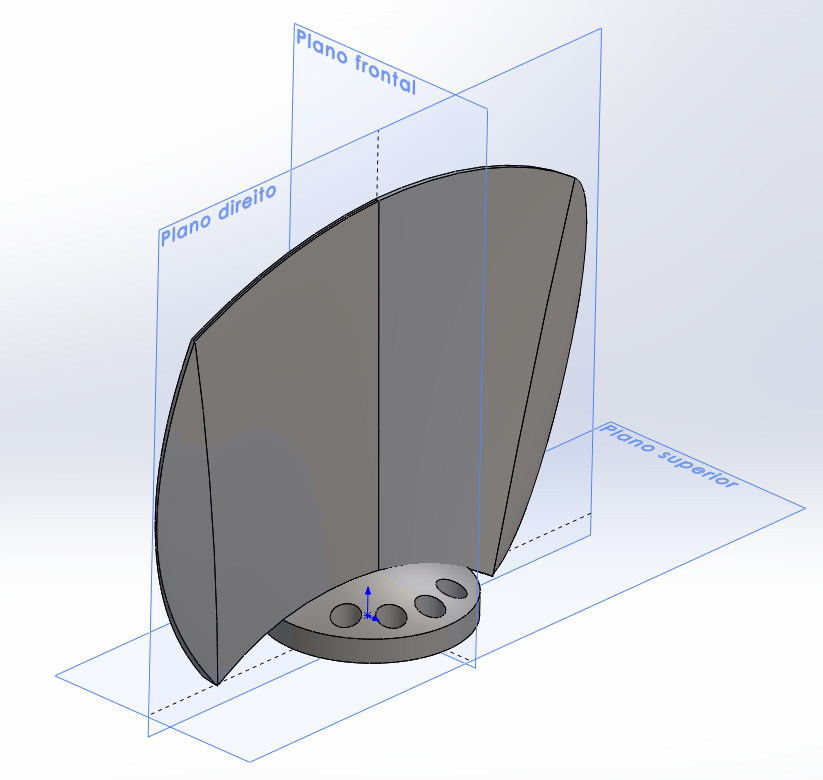
\includegraphics[width=\columnwidth]{figs/bighatch/PaPlanos.PNG}
	\caption{Ilustração das projeções da pá em planos.}
	\label{fig::paplanos}
\end{figure}

\paragraph{KR 10 R1100 sixx WP (Kuka)}
A figura~\ref{fig::kukageom} ilustra a interseção do espaço de trabalho
simplificado do manipulador Kuka KR10 e a projeção da pá. No
caso do Kuka KR 10 R1100, o raio da esfera é aproximado a $\overline{OB^i} = $
alcance do manipulador + comprimento da pistola + 230 mm $= $. 

\begin{figure}[h!]	
	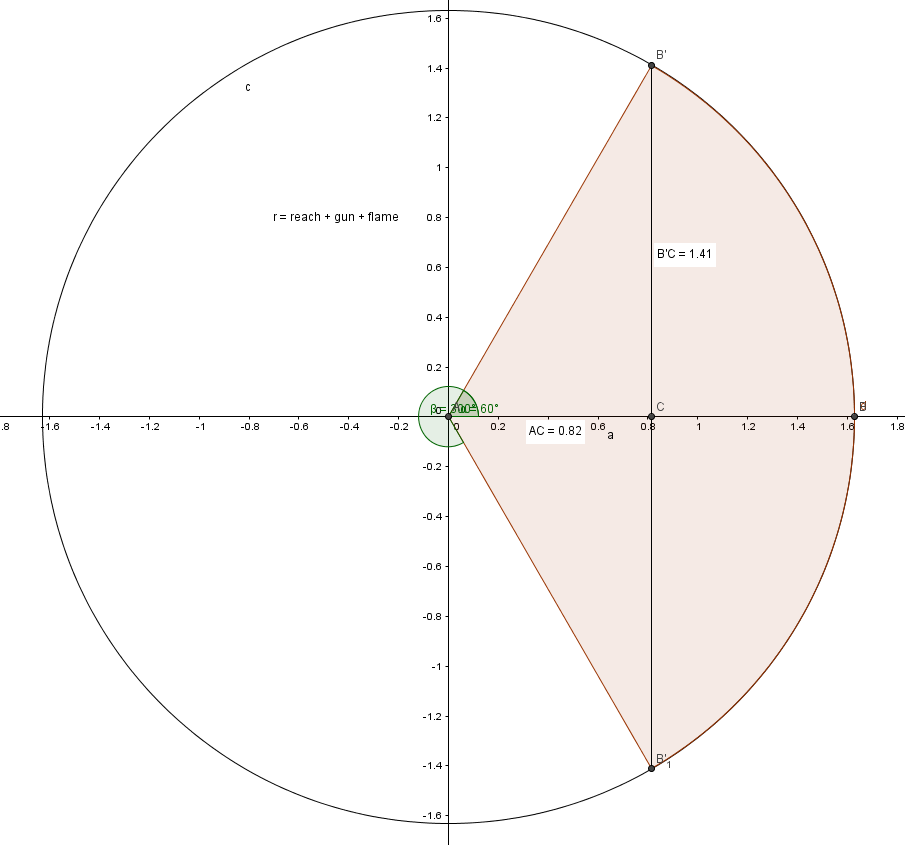
\includegraphics[width=\columnwidth]{figs/bighatch/kukageom.jpg}
	\caption{Ilustração da interseção do espaço de trabalho simplificado do
	manipulador Kuka KR10 e a projeção da pá.}
	\label{fig::kukageom}
\end{figure}

\paragraph{MH12 (Motoman)}

\begin{figure}[h!]	
	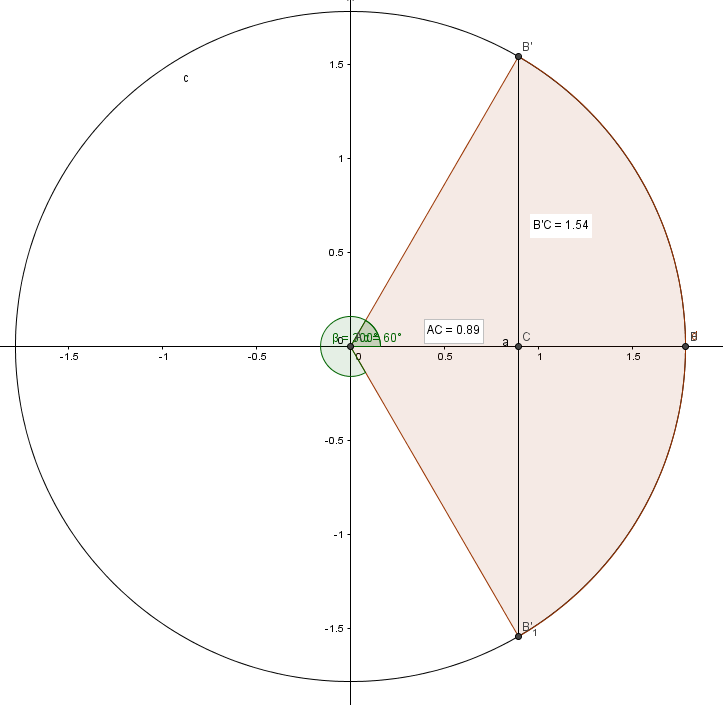
\includegraphics[width=\columnwidth]{figs/bighatch/motomangeom.jpg}
	\caption{Ilustração da interseção do espaço de trabalho simplificado do
	manipulador Motoman MH12 e a projeção da pá.}
	\label{fig::motomangeom}
\end{figure}
\subsubsection{Espaço de trabalho e cinemática do manipulador}
Como já mencionado, o ambiente de simulação foi desenvolvido utilizando a
arquitetura de planejamento Openrave. Para cada manipulador selecionado após a
pesquisa de mercado, serão analisados os reais espaços de trabalho, e o processo de
revestimento da pá em um ambiente simulado que representa as principais
caracterísiticas do ambiente real.

Para gerar o espaço de trabalho, o Openrave utiliza um método de força bruta,
onde são executadas iterações sob iterações de todas as juntas, por seus ângulos
limites e com o passo de ângulo dependendo da resolução do manipulador. O grau
de manipulabilidade do robô é representado por um gradiente de cores, cujo grau
varia do azul claro (menor manipulabilidade) ao vermelho escuro (maior manipulabilidade).
Entende-se por manipulabilidade a capacidade que o robô possui de manipular
objetos em direções específicas, isto é, para uma posição específica é
possível alcançar variadas orientações. Em todas as simulações, a pistola foi
representada como um cilindro de comprimento 300 mm e raio 50 mm, e o efetuador está no extremo do cilindro.

A superfície da pá é amostrada, formando uma grade de tamanho fixo. A técnica
\textit{axis-aligned bounding box (AABB)} é utilizada para obter os
pontos e suas respectivas normais, na superfície da pá. Nesta técnica, a
superfície alvo é inscrita em um bloco, que é uniformemente amostrado. É, então,
realizada uma verificação de colisão entre os pontos amostrados no bloco e a
superfície alvo e, caso haja interseção, o ponto é armazenado junto com sua
normal à superfície. Dessa forma, podemos amostrar a pá e deslocar estes pontos
230 mm em relação à sua normal com a superfície, garantindo a requerimento do
revestimento. A representação dos pontos amostrados e deslocados em relação às
normais da pá podem estão nas figuras~\ref{fig::amostrapa1} e ~\ref{fig::amostrapa2}. 

Utilizando as informações dos pontos amostrados e o espaço de trabalho do
manipulador, foram gerados scripts para calcular a
melhor distância do manipulador em relação a pá, de forma que o maior número de
pontos revestidos com angulação de $90^o$ fossem cobertos.
Essa distância é calculada em relação à normal da pá. Com esse dado, é possível estimar quantas posições da base do
manipulador serão necessários para o revestimento de toda a pá.

\begin{figure}[h!]	
	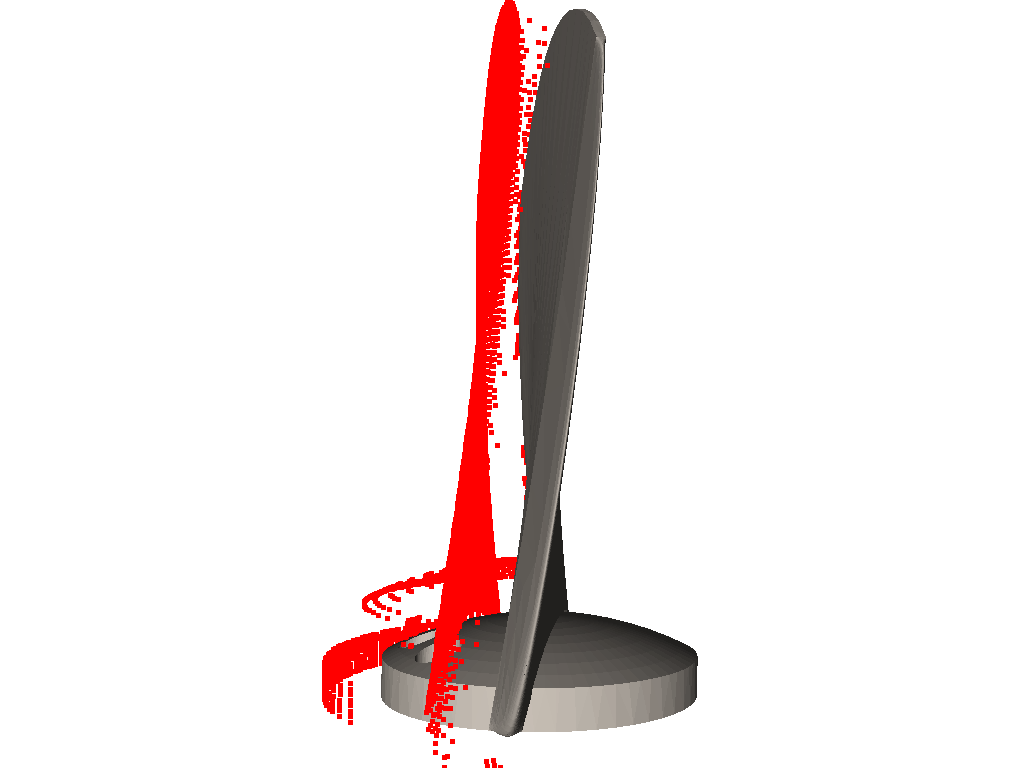
\includegraphics[width=\columnwidth]{figs/bighatch/amostrapa1.png}
	\caption{Pontos amostrados da pá - vista lateral}
	\label{fig::amostrapa1}
\end{figure}

\begin{figure}[h!]	
	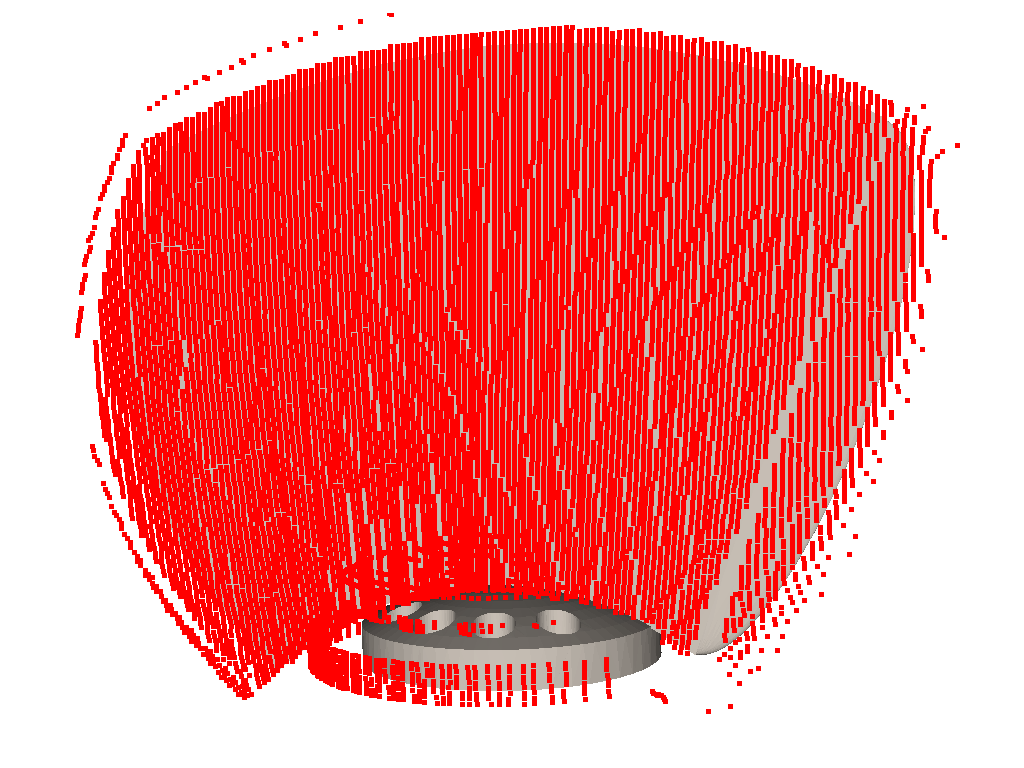
\includegraphics[width=\columnwidth]{figs/bighatch/amostrapa2.png}
	\caption{Pontos amostrados da pá - vista frontal}
	\label{fig::amostrapa2}
\end{figure}

As tabelas~\ref{tab::robocarac} e ~\ref{tab::robocarac} abaixo resume as
caracterísitcas de cada robô e o estudo cinemático realizado, respectivamente:

\begin{center}
\begin{tabular}{  c | c | c | c  }
  \hline
  \textbf{Robô} & \textbf{Payload (Kg)} & \textbf{Massa (Kg)} & \textbf{Alcance
  (mm)} \\ \hline 
  KR10 & 10 & 56 & 1100 \\ \hline
  MH12 & 20 & 130 & 2551  \\ \hline
  LBR 14 & 14 & 30 & 820 \\ \hline
  SIA20D & 20 & 120 &  910 \\
  \hline
\end{tabular}
\captionof{table}{Caracterísitcas principais dos robôs.}
\label{tab::robocarac}
\end{center}

\begin{center}
\begin{tabular}{  c | c | c }
  \hline
  \textbf{Robô} & \textbf{Pontos revestidos (\%)} & \textbf{Posições de base} \\ \hline 
  KR10 & 24.33 & 13\\ \hline 
  MH12 & 53.3 & 4   \\ \hline
  LBR 14 $\uparrow$ & 17.2 & 13 \\ \hline
  LBR 14 $\rightarrow$ & 17.37 & 13 \\ \hline
  SIA20D $\uparrow$ & 23.14 & 9 \\ \hline
  SIA20D $\rightarrow$ & 24.76 & 9 \\ 
  \hline
\end{tabular}
\captionof{table}{Resumo do estudo
cinemático.}
\label{tab::robocin}
\end{center}

\paragraph{KR 10 R1100 sixx WP (Kuka)}
A figura~\ref{fig::kr10cin1} e figura~\ref{fig::kr10cin2} mostram as vistas
lateral e superior do espaço de trabalho do manipulador, respectivamente. Em
vermelho, estão representados os pontos a serem revestidos e em preto os pontos
que o manipulador foi capaz de revestir.

O script que calcula a melhor posição da base em relaçao à pá retornou a posição
870 mm, sendo que 3825 pontos foram revestidos, representando 24.33\% de toda a
pá. Estima-se que serão necessários, pelo menos, 13 posições para o recobrimento
de toda a pá, figura~\ref{fig::kr10bestpos}.



\begin{figure}[h!]	
	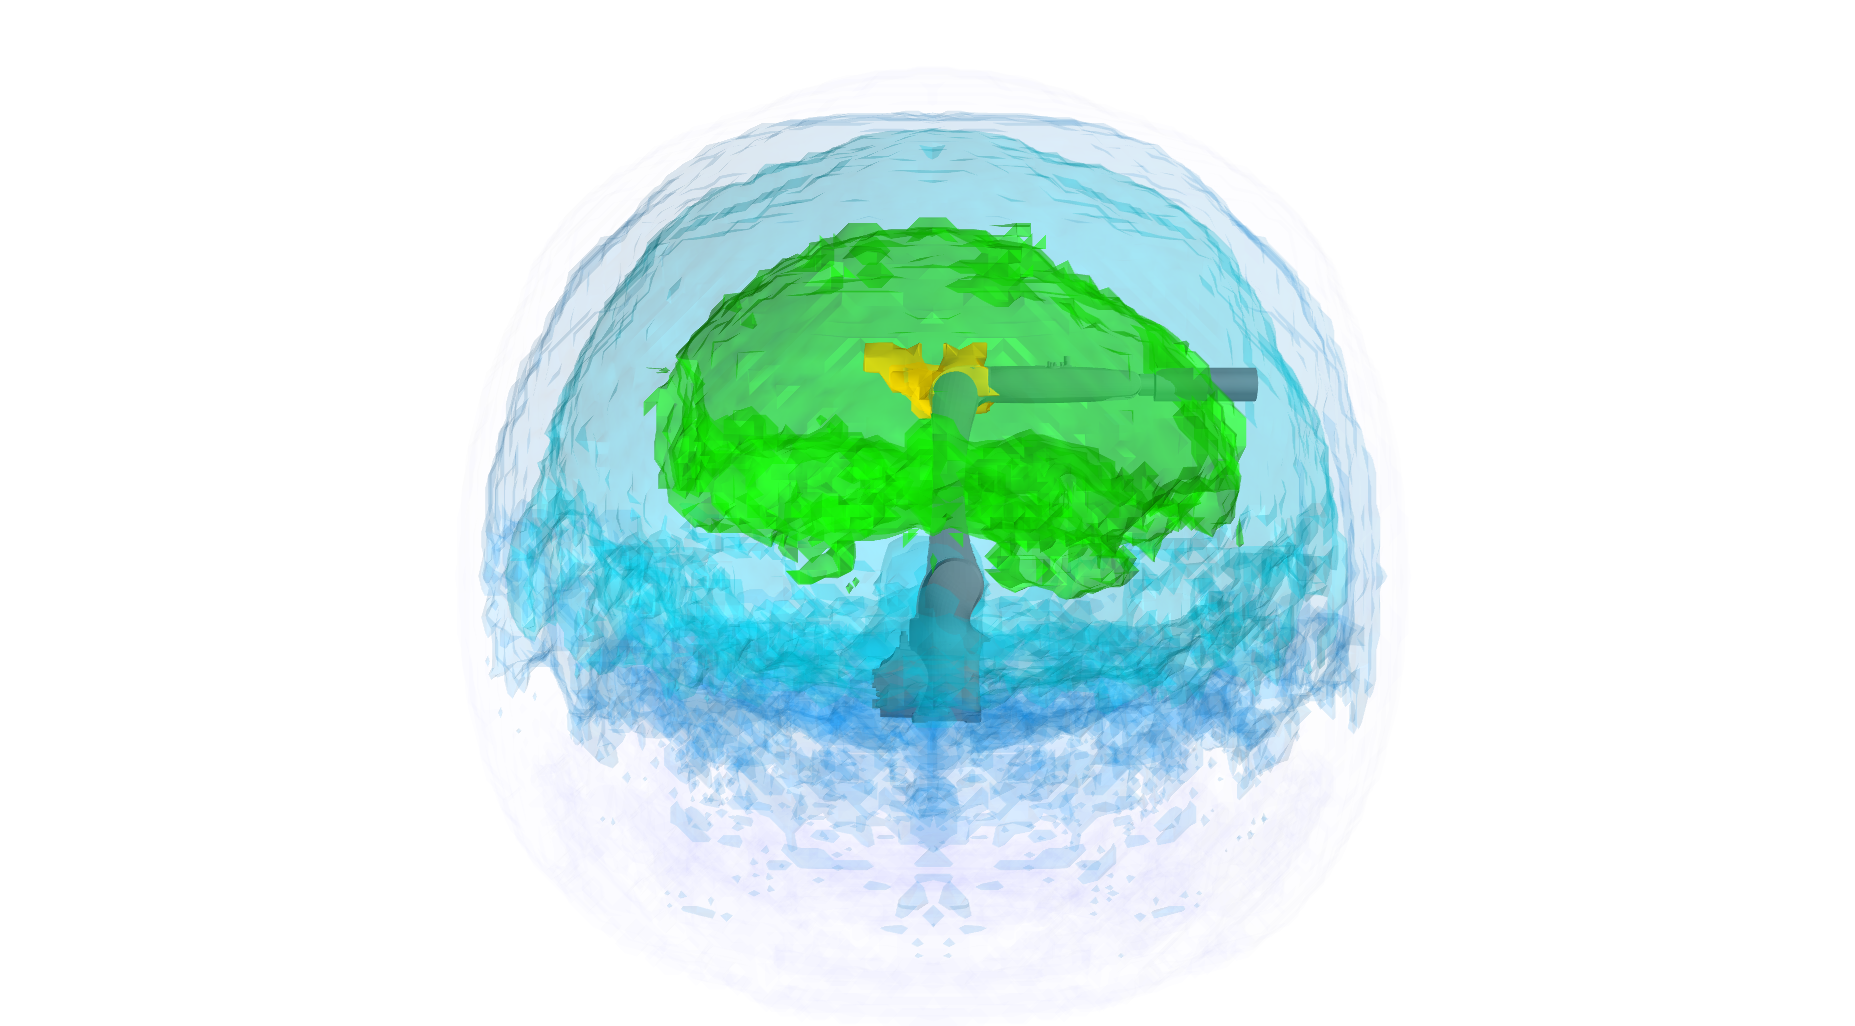
\includegraphics[width=\columnwidth]{figs/bighatch/kr10_front.png}
	\caption{Espaço de trabalho do manipulador Kuka KR10 - vista lateral}
	\label{fig::kr10cin1}
\end{figure}

\begin{figure}[h!]	
	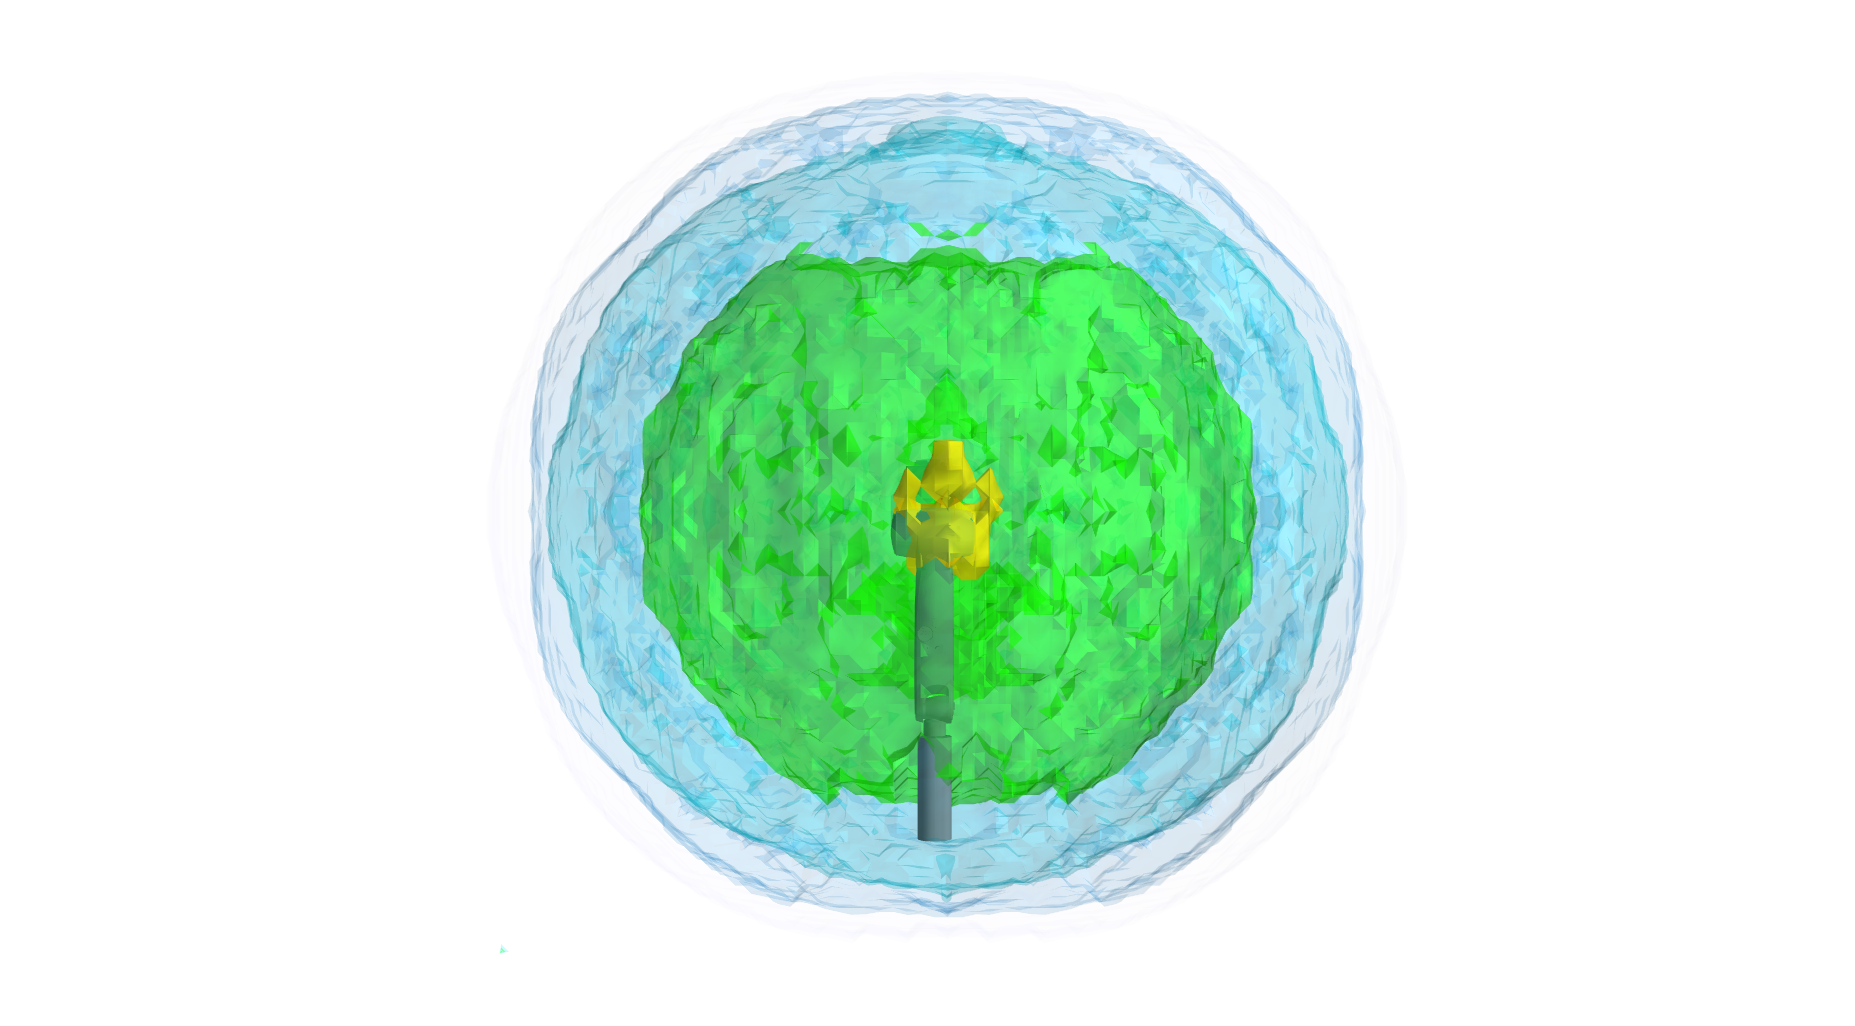
\includegraphics[width=\columnwidth]{figs/bighatch/kr10_top.png}
	\caption{Espaço de trabalho do manipulador Kuka KR10 - vista superior}
	\label{fig::kr10cin2}
\end{figure}

\begin{figure}[h!]	
	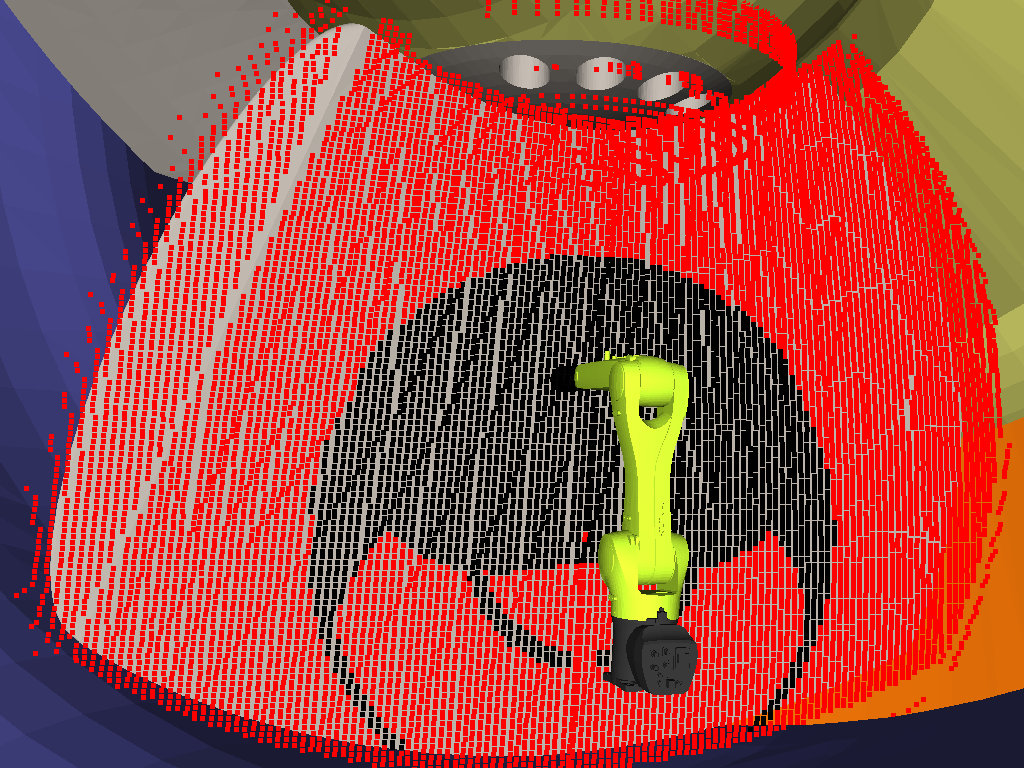
\includegraphics[width=\columnwidth]{figs/bighatch/kr10_bestpos.png}
	\caption{Melhor posição para o revestimento - robô KR10 da Kuka.}
	\label{fig::kr10bestpos}
\end{figure}


\paragraph{MH12 (Motoman)}
A figura~\ref{fig::mh12cin1} e figura~\ref{fig::mh12cin2} mostram as vistas
lateral e superior do espaço de trabalho do manipulador, respectivamente.

O script que calcula a melhor posição da base em relaçao à pá retornou a posição
950 mm, sendo que 8379 pontos foram revestidos, representando 53.30\% de toda a
pá. Estima-se que serão necessários, pelo menos, 4 posições para o recobrimento
de toda a pá, figura~\ref{fig::mh12bestpos}.

\begin{figure}[h!]	
	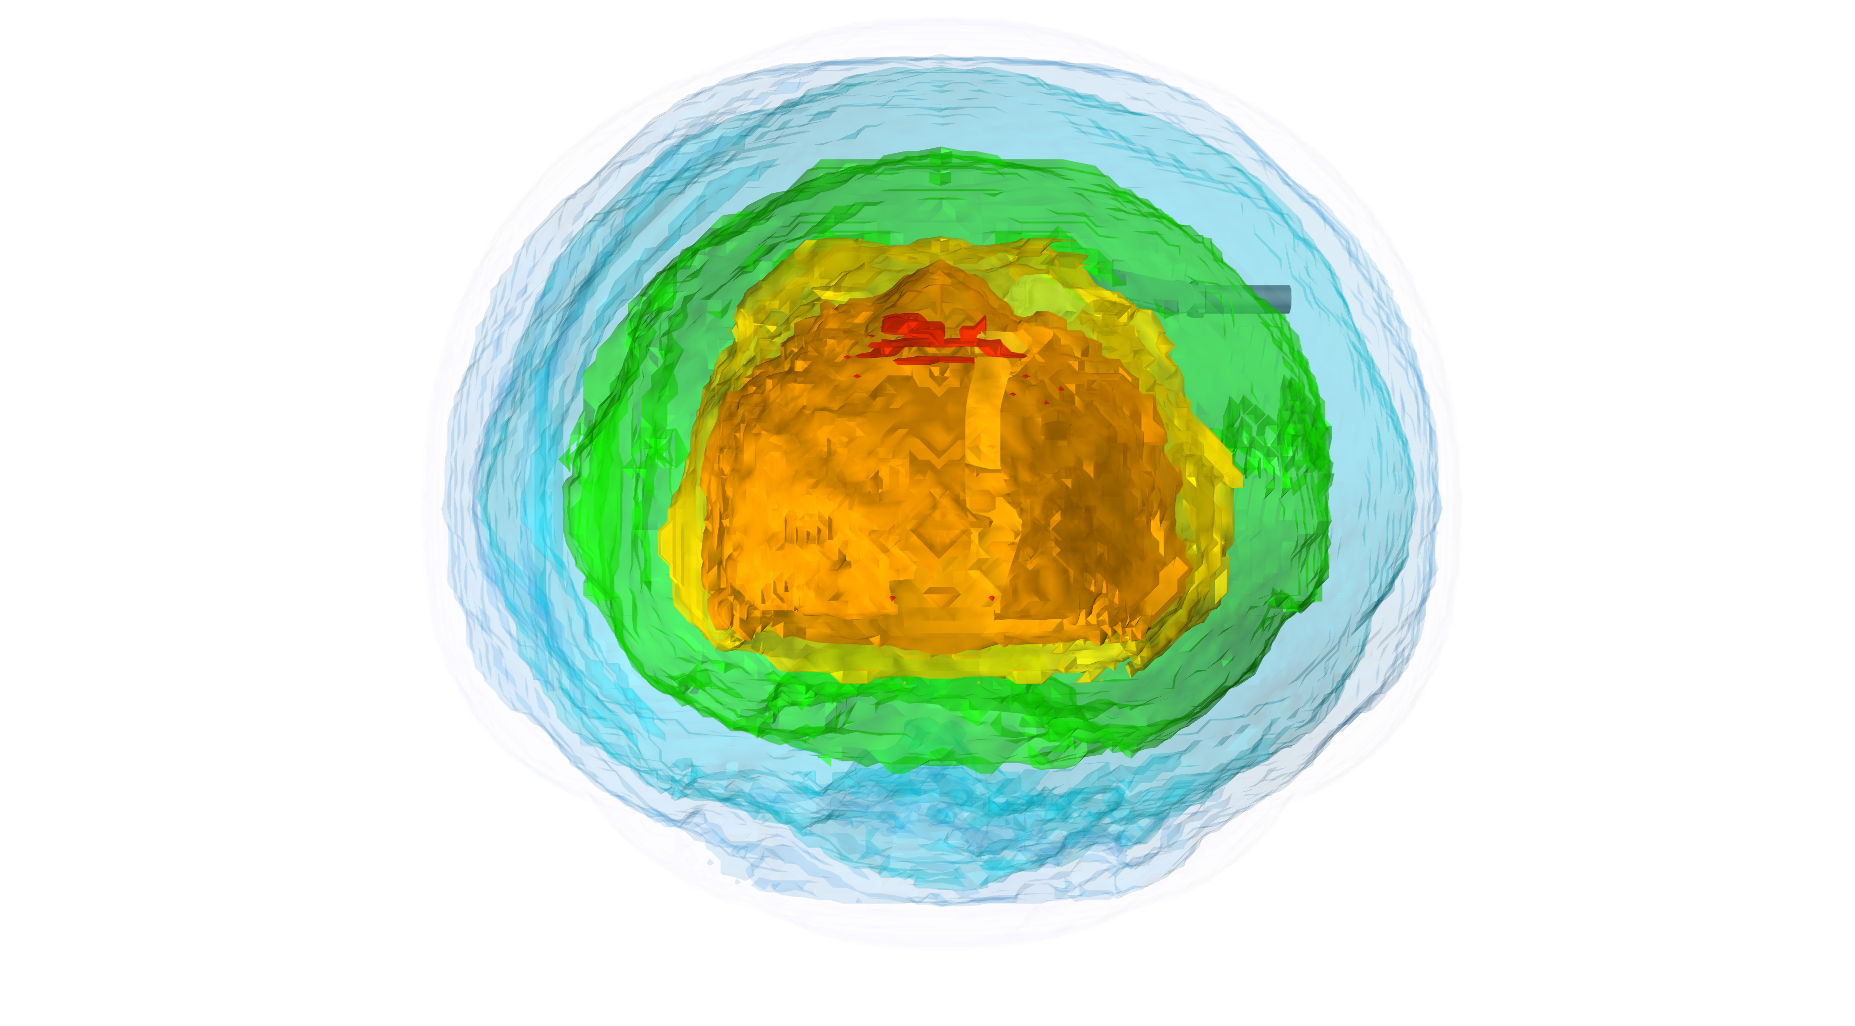
\includegraphics[width=\columnwidth]{figs/bighatch/mh12_front.png}
	\caption{Espaço de trabalho do manipulador MH12 - vista lateral}
	\label{fig::mh12cin1}
\end{figure}

\begin{figure}[h!]	
	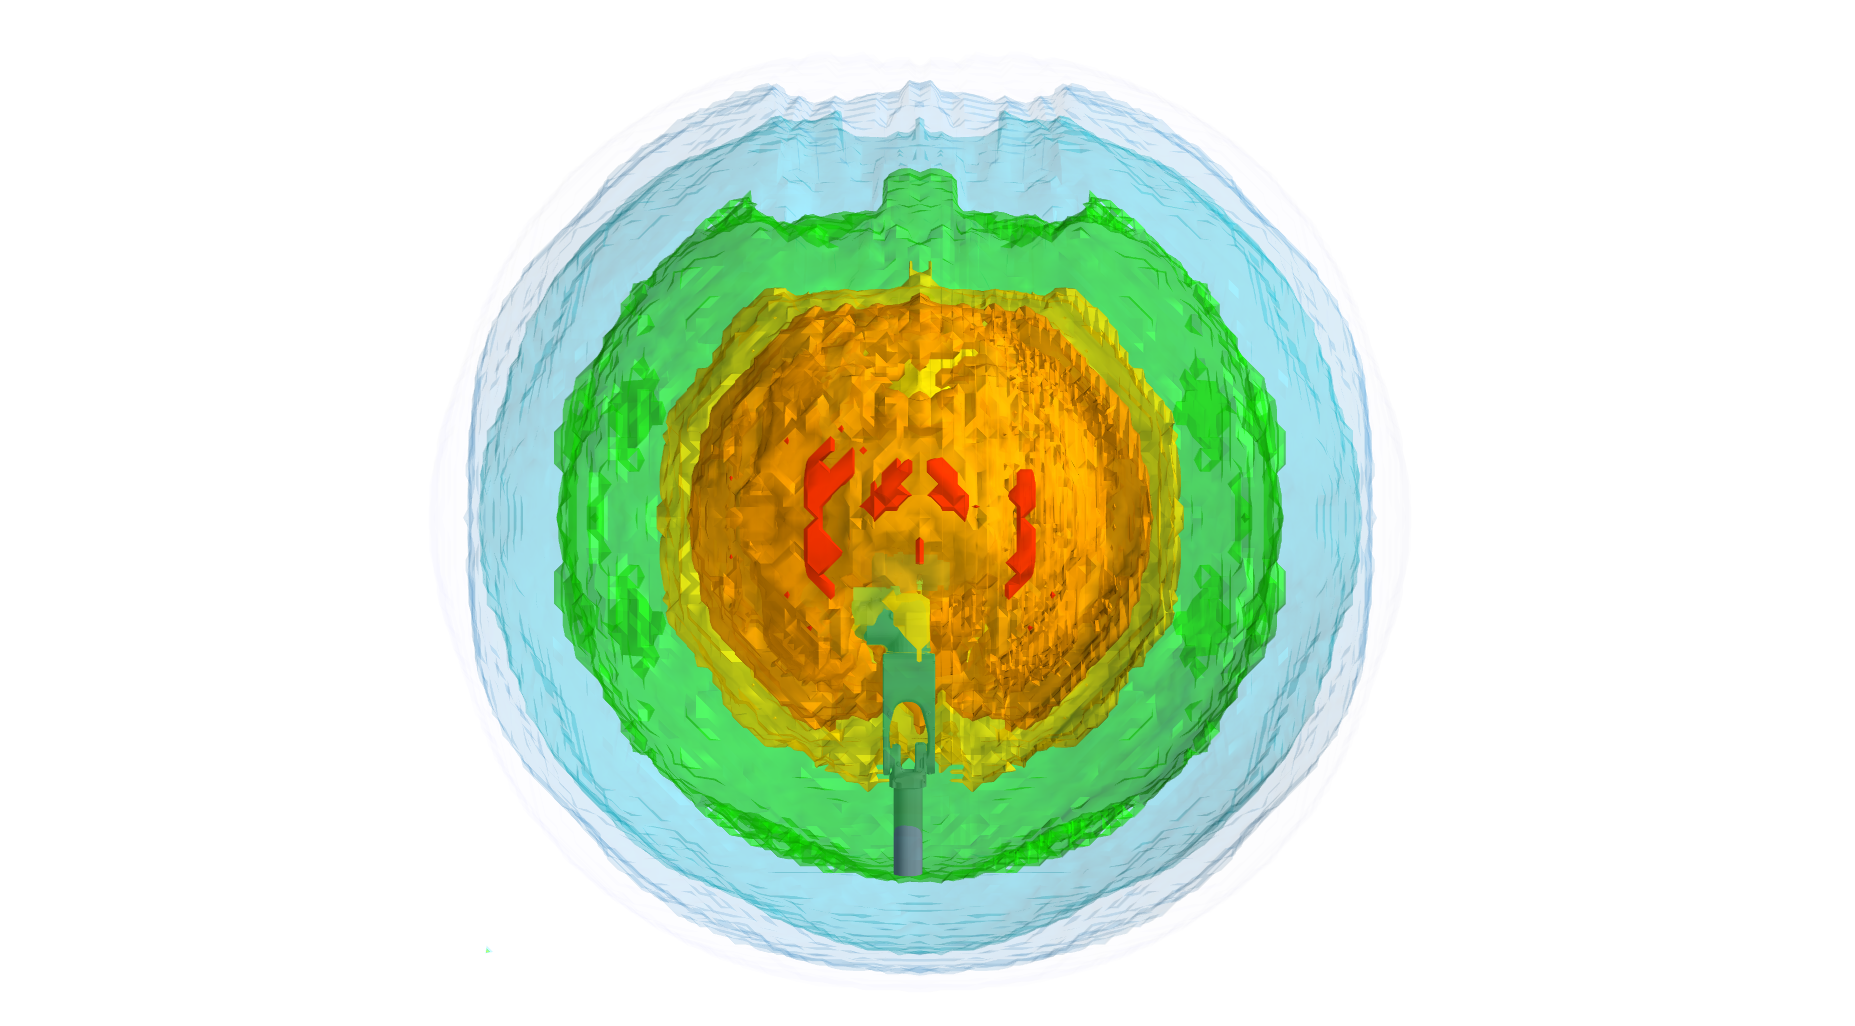
\includegraphics[width=\columnwidth]{figs/bighatch/mh12_top.png}
	\caption{Espaço de trabalho do manipulador MH12 - vista superior}
	\label{fig::mh12cin2}
\end{figure}

\begin{figure}[h!]	
	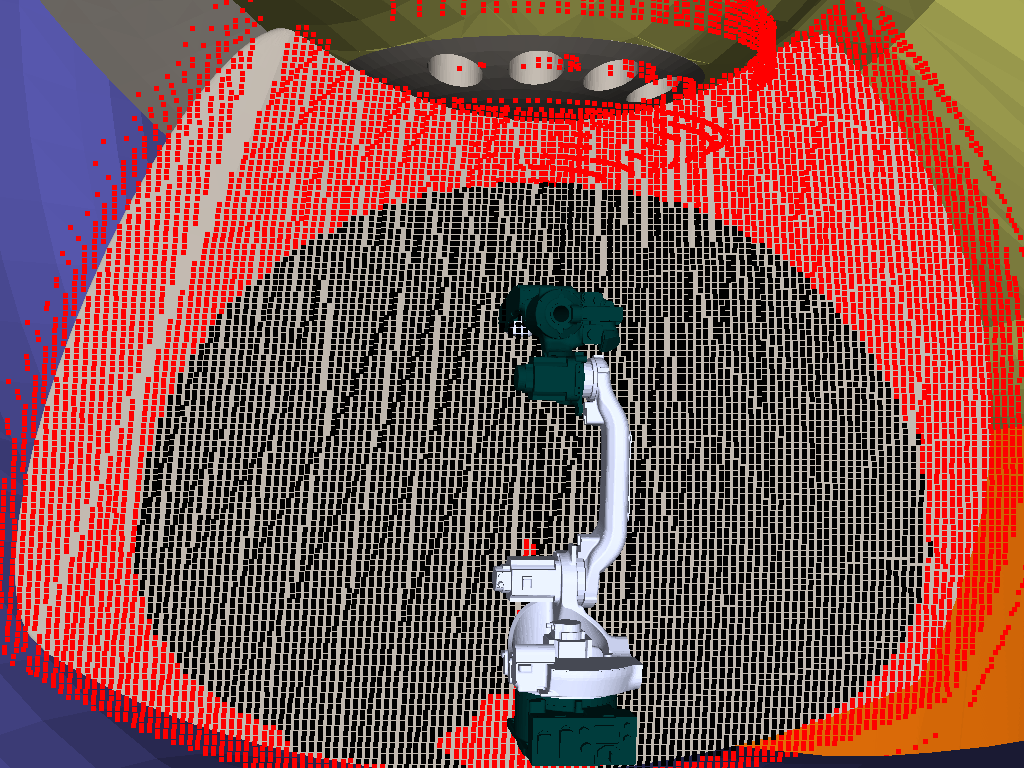
\includegraphics[width=\columnwidth]{figs/bighatch/mh12_bestpos.png}
	\caption{Melhor posição para o revestimento - robô MH12 da Motoman.}
	\label{fig::mh12bestpos}
\end{figure}


\paragraph{LBR iiwa 14 R820 (Kuka)}
O manipulador LBR iiwa 14 R820 possui 7 graus de liberdade e, devido a sua
grande flexibilidade e facilidade de montagem, foram estudadas duas
configurações para a base.

O script que calcula a melhor posição da base na posição vertical em relaçao à
pá retornou a posição 1.06, sendo que 2648 pontos foram revestidos,
representando 17.20\% de toda a pá. Estima-se que serão necessários, pelo menos,
13 posições para o recobrimento de toda a pá, figura~\ref{fig::lbrbestposv}.

\begin{figure}[h!]	
	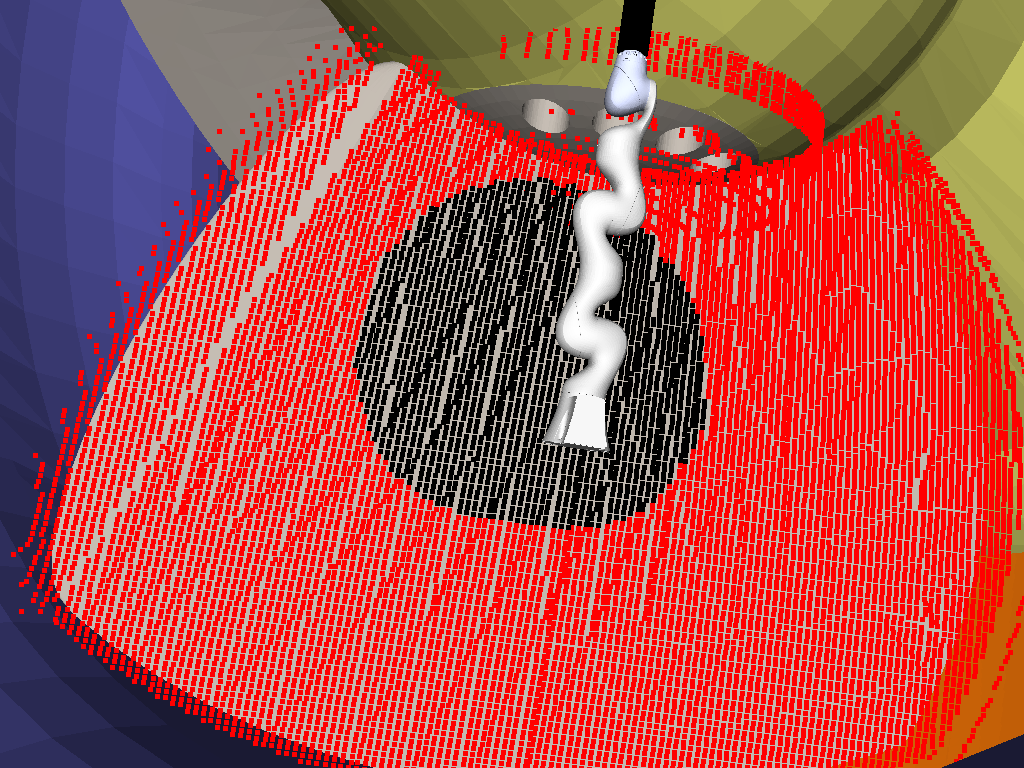
\includegraphics[width=\columnwidth]{figs/bighatch/lbr_bestposv.png}
	\caption{Melhor posição para o revestimento - robô LBR da Kuka com base na
	posição vertical.}
	\label{fig::lbrbestposv}
\end{figure}

O script que calcula a melhor posição da base na posição vertical em relaçao à
pá retornou a posição 1400 mm, sendo que 2730 pontos foram revestidos,
representando 17.37\% de toda a pá. Estima-se que serão necessários, pelo menos,
13 posições para o recobrimento de toda a pá, figura~\ref{fig::lbrbestposh}.

\begin{figure}[h!]	
	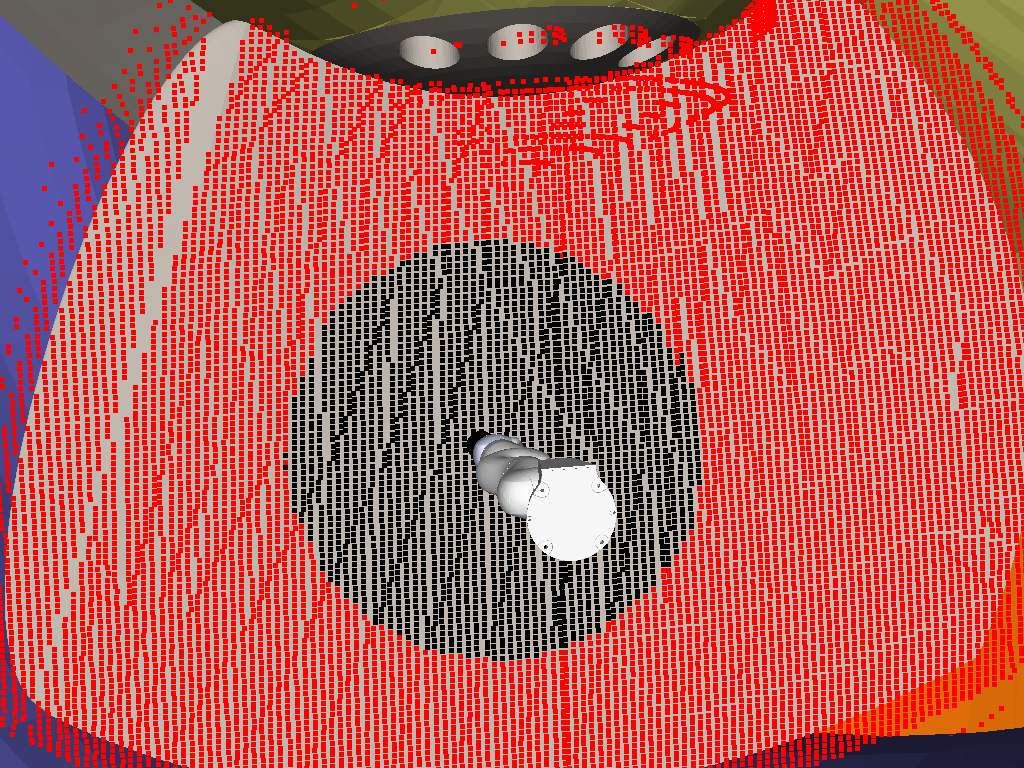
\includegraphics[width=\columnwidth]{figs/bighatch/lbr_bestposh.png}
	\caption{Melhor posição para o revestimento - robô LBR da Kuka com base na
	posição horizontal.}
	\label{fig::lbrbestposh}
\end{figure}

\paragraph{SIA20D (Motoman)}
O manipulador SIA20D também possui 7 graus de liberdade e, devido a sua
grande flexibilidade e facilidade de montagem, foram estudadas duas
configurações para a base.

O script que calcula a melhor posição da base na posição vertical em relaçao à
pá retornou a posição 1100 mm, sendo que 3638 pontos foram revestidos,
representando 23.14\% de toda a pá. Estima-se que serão necessários, pelo menos,
9 posições para o recobrimento de toda a pá, figura~\ref{fig::sia20dbestposv}.

\begin{figure}[h!]	
	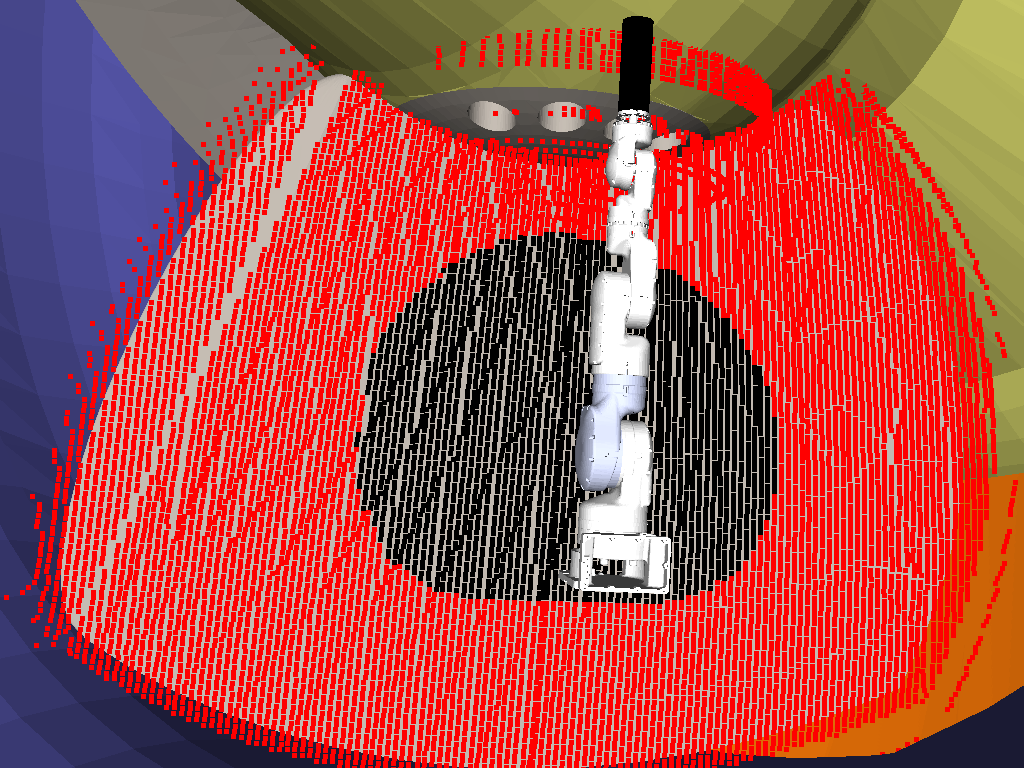
\includegraphics[width=\columnwidth]{figs/bighatch/sia20d_bestposv.png}
	\caption{Melhor posição para o revestimento - robô SIA20D da Motoman com base
	na posição vertical.}
	\label{fig::sia20dbestposv}
\end{figure}

O script que calcula a melhor posição da base na posição horizontal em relaçao à
pá retornou a posição 1510 mm, sendo que 3892 pontos foram revestidos,
representando 24.76\% de toda a pá. Estima-se que serão necessários, pelo menos,
9 posições para o recobrimento de toda a pá, figura~\ref{fig::sia20dbestposh}.

\begin{figure}[h!]	
	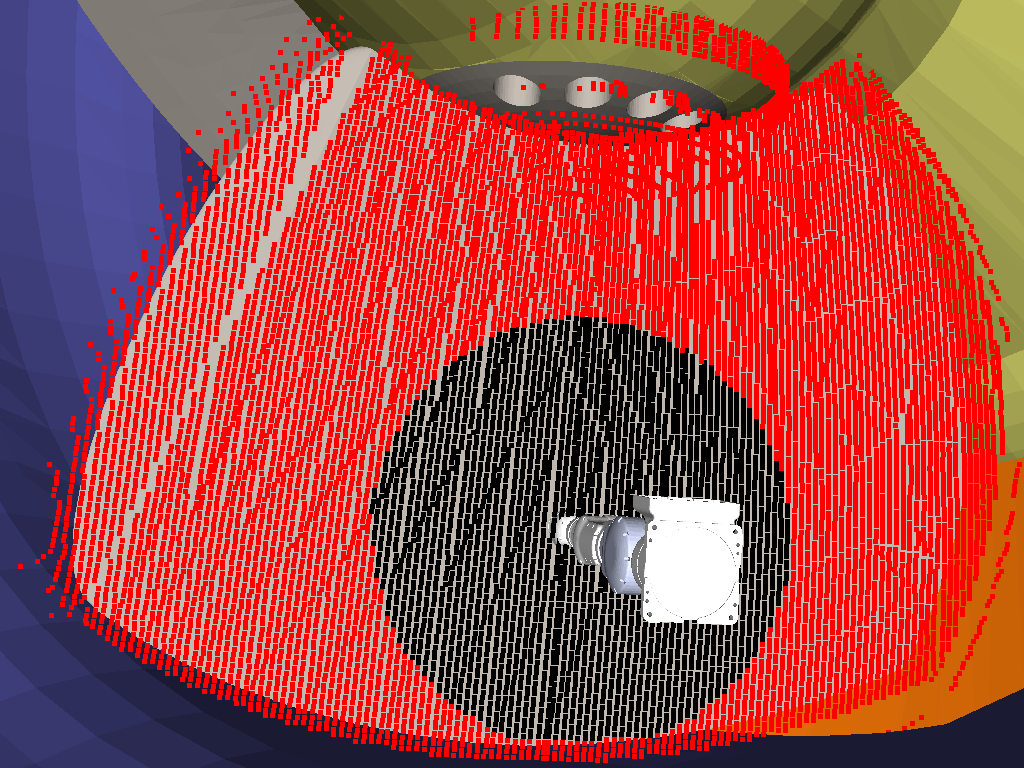
\includegraphics[width=\columnwidth]{figs/bighatch/sia20d_bestposh.png}
	\caption{Melhor posição para o revestimento - robô SIA20D da Motoman com base
	na posição horizontal.}
	\label{fig::sia20dbestposh}
\end{figure}

\paragraph{Tolerância no ângulo de revestimento}
As análises de revestimento dos manipuladores exigiram que a pistola
estivesse com as mesmas direções e sentidos opostos às normais dos
pontos a serem revestidos, isto é, a orientação da pistola é sempre
perpendicular ao plano da pá. Entretanto, pode-se assumir uma tolerância de
$90^o \pm 60^o$ entre a pistola e o plano perpendicular, que foi considerada
na análise puramente geométrica. Como o manipulador MH12 (Motoman) possui
recobrimento de quase todo o alcance vertical da pá (revestimento de cima a
baixo), mostra-se interressante a análise de tolerância neste manipulador, de
forma que haja simplificação das possíveis soluções de bases.

Primeiramente, são armazenados os pontos que o robô não foi capaz de
revestir (pontos em vermelho, nas figuras de espaço de trabalho dos
manipuladores) e suas respectivas normais aos planos tangentes à superfície da
pá. Os pontos são deslocados 230 mm na mesma direção e sentido oposto às suas
respectivas normais, de forma que pertençam à superfície da pá,
ponto $D$ é deslocado até ponto $C$ na figura~\ref{fig::tolerancia1}. Para cada
ponto não revestido, são gerados dois vetores unitários $\overrightarrow{v}$ e
$\overrightarrow{w}$ ortogonais entre si e ao vetor normal $\overrightarrow{N}$,
no plano tangente à superfície da pá conforme
ilustrado na figura~\ref{fig::tolerancia2}. O vetor $\overrightarrow{N}$ é
girado pelo ângulo de tolerância de revestimento $\theta$ (entre $0^o$ e $60^o$)
em relação ao vetor $\overrightarrow{w}$, gerando o vetor
$\overrightarrow{P_1}$, figura~\ref{fig::tolerancia3}.

\begin{figure}[h!]	
	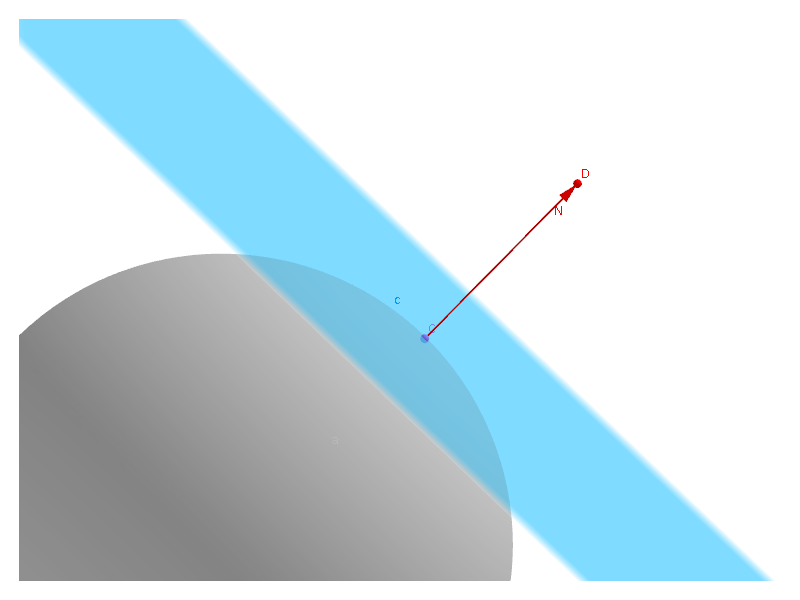
\includegraphics[width=\columnwidth]{figs/bighatch/tolerancia1.png}
	\caption{Ponto D não revestido, deslocado 230 mm da superfície da pá.}
	\label{fig::tolerancia1}
\end{figure}

\begin{figure}[h!]	
	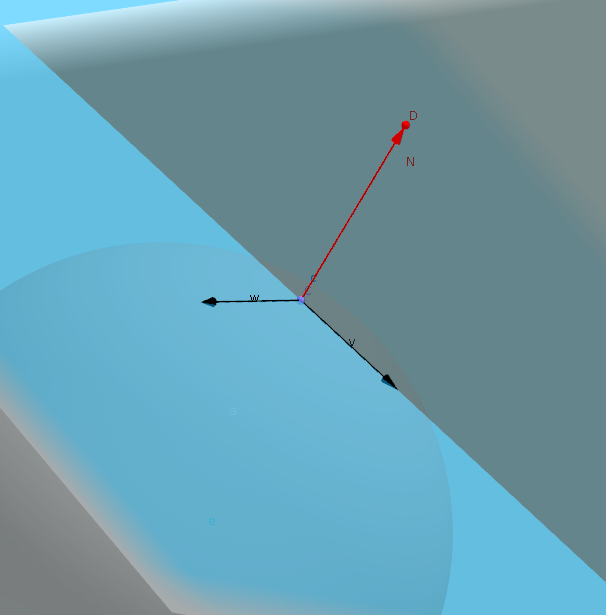
\includegraphics[width=\columnwidth]{figs/bighatch/tolerancia2.png}
	\caption{Vetores v e w ortogonais ao vetor normal N.}
	\label{fig::tolerancia2}
\end{figure}

Finalmente, o vetor $\overrightarrow{P_1}$ pode ser girado em relação a
$\overrightarrow{N}$ e todos os vetores que pertencem à tolerância de
revestimento $\theta$ saem do ponto $C$ até um ponto do círculo $h$, como o
vetor exemplo $\overrightarrow{P_2}$, na figura~\ref{fig::tolerancia4}. Observe
que este círculo deve ser discretizado, e cada ponto pertencente ao círculo e sua
respectiva normal (vetor de origem $C$ ao ponto do círculo) devem ser
reavaliados, isto é, verifica-se se o robô alcança o ponto pertencente a $h$ com
pistola de revestivemto apontada a sua respectiva normal.
Se algum ponto do círculo puder ser revestido, o ponto $D$ pode ser considerado
como revestido. No exemplo da figura~\ref{fig::tolerancia4}, o círculo $h$ foi
discretizado em dois pontos $G$ e $H$, e suas normais são $\overrightarrow{P_1}$
e $\overrightarrow{P_2}$, respectivamente. 

\begin{figure}[h!]	
	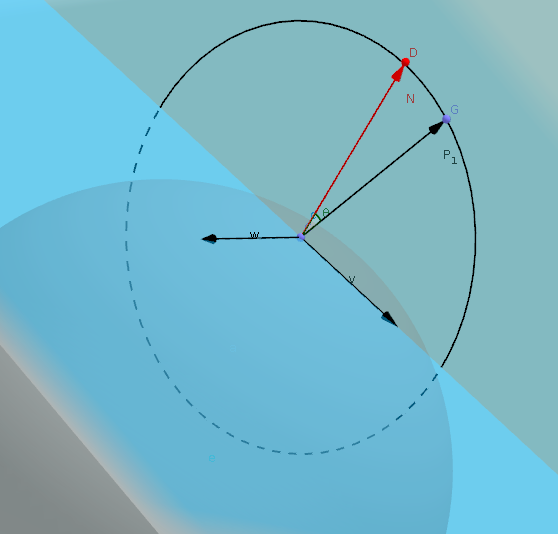
\includegraphics[width=\columnwidth]{figs/bighatch/tolerancia3.png}
	\caption{Vetor N girado pelo ângulo de tolerância de revestimento.}
	\label{fig::tolerancia3}
\end{figure}

\begin{figure}[h!]	
	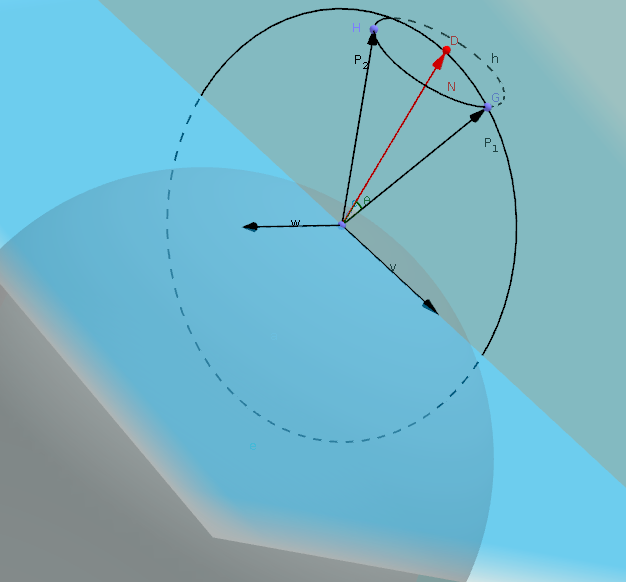
\includegraphics[width=\columnwidth]{figs/bighatch/tolerancia4.png}
	\caption{Circulo $h$ representa todos os pontos equivalentes ao ponto $D$ com
	ângulo de tolerância de revestimento $\theta$.}
	\label{fig::tolerancia4}
\end{figure}

Foram realizadas análises de tolerância para dois robôs: MH12, que apresentou o
maior número de pontos revestido na pá, e LBR R820, que é a única solução viável
de manipulador industrial para o acesso superior. Os ângulos de tolerância foram
variados em $10^o$ e $30^o$. 

\subsubsection{Dinâmica do manipulador}
A dinâmica de um manipulador robótico é a análise de velocidades, acelerações e
torques das juntas. Para esta análise, assume-se que o efetuador, pistola de
revestimento, possui velocidade 40m/min constante em todos os pontos amostrados
da pá. Como velocidades e acelerações exigem a computação de derivadas, é
realizada uma melhor discretização da pá da turbina, na qual o passo de
amostragem é menor e um filtro garante espaçamento uniforme dos pontos de 10 mm.
Para um lado da pá, são amostrados, portanto, 130 mil pontos.

Para cada ponto amostrado da pá, faz-se a análise cinemática e são armazenados
os pontos que são possíveis de serem revestidos, como na
seção~\ref{sec::cinematica}, isto é, são armazenados os pontos que possuem
solução de cinemática inversa. Posteriormente, para cada ponto revestido, é
criado um conjunto contendo seus 8 pontos vizinhos através de um algoritmo k-d
tree, como na figura~\ref{fig::pontosdin}, onde $p_r$ é o ponto de referência a
ser analisado dinamicamente e os pontos ${p_1,p_2,q_1,q_2,r_1,r_2,s_1,s_2}$ são auxiliares
para o estudo. 

\begin{figure}[h!]	
	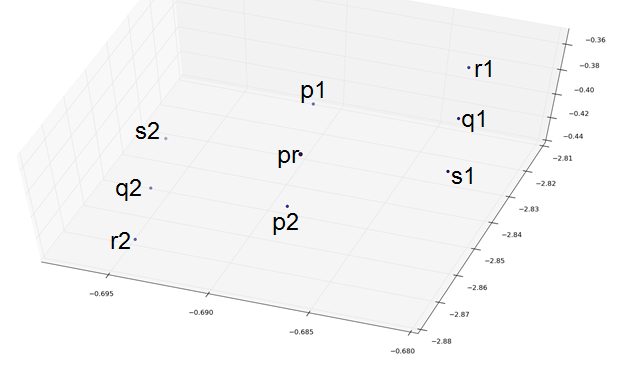
\includegraphics[width=\columnwidth]{figs/dinamica/pontosdinamica.png}
	\caption{Pontos exemplo amostrados da pá.}
	\label{fig::pontosdin}
\end{figure}

%As soluções de cinemática inversa (ângulos das juntas do robô)
%$\Theta_r
%=
%{\theta_{p_r},\theta_{p_1},\theta_{p_2},\theta_{q_1},\theta_{q_2},\theta_{r_1},\theta_{r_2},\theta_{s_1},\theta_{s_2}}$
As velocidades angulares das juntas são calculadas a partir da cinemática
diferencial. Para isso, usa-se o cálculo da matriz jacobiana ($J$), que é a
diferenciação (derivadas parciais) da matriz de cinemática direta em função das
variáveis de junta \citep{sciavicco2000differential}. A velocidade linear do
efetuador ($\dot{X}$) e o jacobiano são conhecidos em cada ponto de referência, logo
podem-se calcular as velocidades das juntas do manipulador entre o ponto de
referência e cada ponto auxiliar: $\dot{X} = J\dot{q}\Rightarrow
J^+\dot{X}=\dot{q}$, onde $J^+$ é a pseudo inversa Moore-Penrose de $J$.

As velocidades angulares são $\Omega_r
=
\{\omega_{p_r,p_1},\omega_{p_r,p_2},\omega_{p_r,q_1},\omega_{p_r,q_2},\omega_{p_r,r_1},\omega_{p_r,r_2},\omega_{p_r,s_1},\omega_{p_r,s_2}\}$,
onde $\omega$, $\omega\in\Omega_r$, é um vetor $n \times 1$, e $n$ é o número de
juntas do robô. As velocidades dos ângulos das juntas é uma informação importate para a
verificação da viabilidade das trajetórias do robô. Para o caso do robô
MH12, onde $\omega_{\textbf{max}}=\{220, 200, 220, 410, 410, 610\}^o/s$, por
exemplo, caso não haja $\omega\in\Omega_r$, tal que
$\omega\leq\omega_{\textbf{max}}$, não é possível realizar o revestimento do
ponto de referência $p_r$. Se $\exists \omega\in\Omega_r$ tal que
$\omega\leq\omega_{\textbf{max}}$, o ponto de referência é viável pela
cinemática inversa e pela cinemática diferencial, mas pode ser inviável ainda
pela análise dinâmica, que considera as acelerações, massas e forças do
conjunto.

As equações dinâmicas de um manipulador são também abordados em
\cite{sciavicco2000differential} e possuem duas abordagens bem conhecidas na
literatura: equações de Newton-Euler e equações de Lagrange. O ambiente OpenRave
utiliza o método de Newton-Euler para computar os torques das juntas (dinâmica
inversa): $\tau = M(q)\alpha + C(q,\omega)\omega + G(q) $, onde $\tau$ é o
vetor de torques das juntas, $M$ matriz de massas e momentos de inércia,
$\alpha$ é acelerações das juntas, $C$ matriz de Coriolis, $\omega$ é as
velocidades das juntas e $G$ o vetor de gravidade.

Para a formação da matriz $M$, é necessária a estimação de parâmetros do
manipulador. A estimação dos parâmetros pode ser realizada de maneira iterativa,
isto é, aplicam-se torques nas juntas e, pela resposta
do manipulador, estima-se a matriz \citep{slotine1988adaptive}; ou pelo CAD do
manipulador, por exemplo, pela utilização da ferramenta SolidWorks. Foi utilizado o método de estimação pelo CAD do
manipulador, visto que os manipuladores ainda estavam em estudo e não foram
adquiridos, além disso houve facilidade de aproximar os parâmetros já que o CAD
fornecido pelo fabricante é bem detalhado. 

A aceleração angular, $\alpha$, é necessária para a computação dos torques,
$\tau$. O método analítico para cálculo da aceleração angular das juntas é
através da derivada da equação da cinemática diferencial:
$\ddot{X}=\dot{q}^TH\dot{q}+J\ddot{q} \Rightarrow
\ddot{q}=J^+(\ddot{X}-\dot{q}^TH\dot{q})$ ou
$\alpha=J^+(a-\omega^TH\omega)$, onde $H$ é a matriz Hessiana, isto é, derivada
parcial da matriz jacobiana $J$ \citep{hourtash2005kinematic}. 

Com a informação dos ângulos, velocidades e acelerações das juntas, momentos
de inércia e massa dos elos, o OpenRave calcula a dinâmica inversa através do
método Newton-Euler, obtendo-se os torques. Para cada ponto de referência, há quatro direções
(trajetórias) possíveis amostradas que o efetuador pode percorrer:
$\{(p_1,p_r,p_2),(q_1,p_r,q_2),(r_1,p_r,r_2),(s_1,p_r,s_2)\}$, logo quatro
ângulos, velocidades e acelerações de juntas, portanto são obtidos quatro
possíveis vetores de torques:
$T=\{\tau_{rp},\tau_{rq},\tau_{rr},\tau_{rs}\}$. E, especificamente para o
caso do manipulador MH12, os valores dos torques devem ser inferiores aos
estabelecidos pelo datasheet:
$\tau_{\textbf{max}}=\{-,-,-,22,22,9.8\}\textbf{Nm}$, logo se $\exists \tau\in
T$, tal que $\tau\leq\tau_{\textbf{max}}$, então há uma trajetória viável.

As figuras~\ref{fig::wgeo}, ~\ref{fig::wcin} e ~\ref{fig::wdin} representam a
evolução das análises do manipulador, de um nível mais simples a um nível mais
complexo de detalhamento, o qual avalia velocidades, acelerações e torques das
juntas do manipulador. Ainda deverá ser executada a análise de manipulabilidade
que avalia o sistema de controle do manipulador. Esta análise é importante para
o planejamento de trajetórias do manipulador e para o cálculo das posições
viáveis da base para uma operação completa.



\begin{figure}[h!]	
	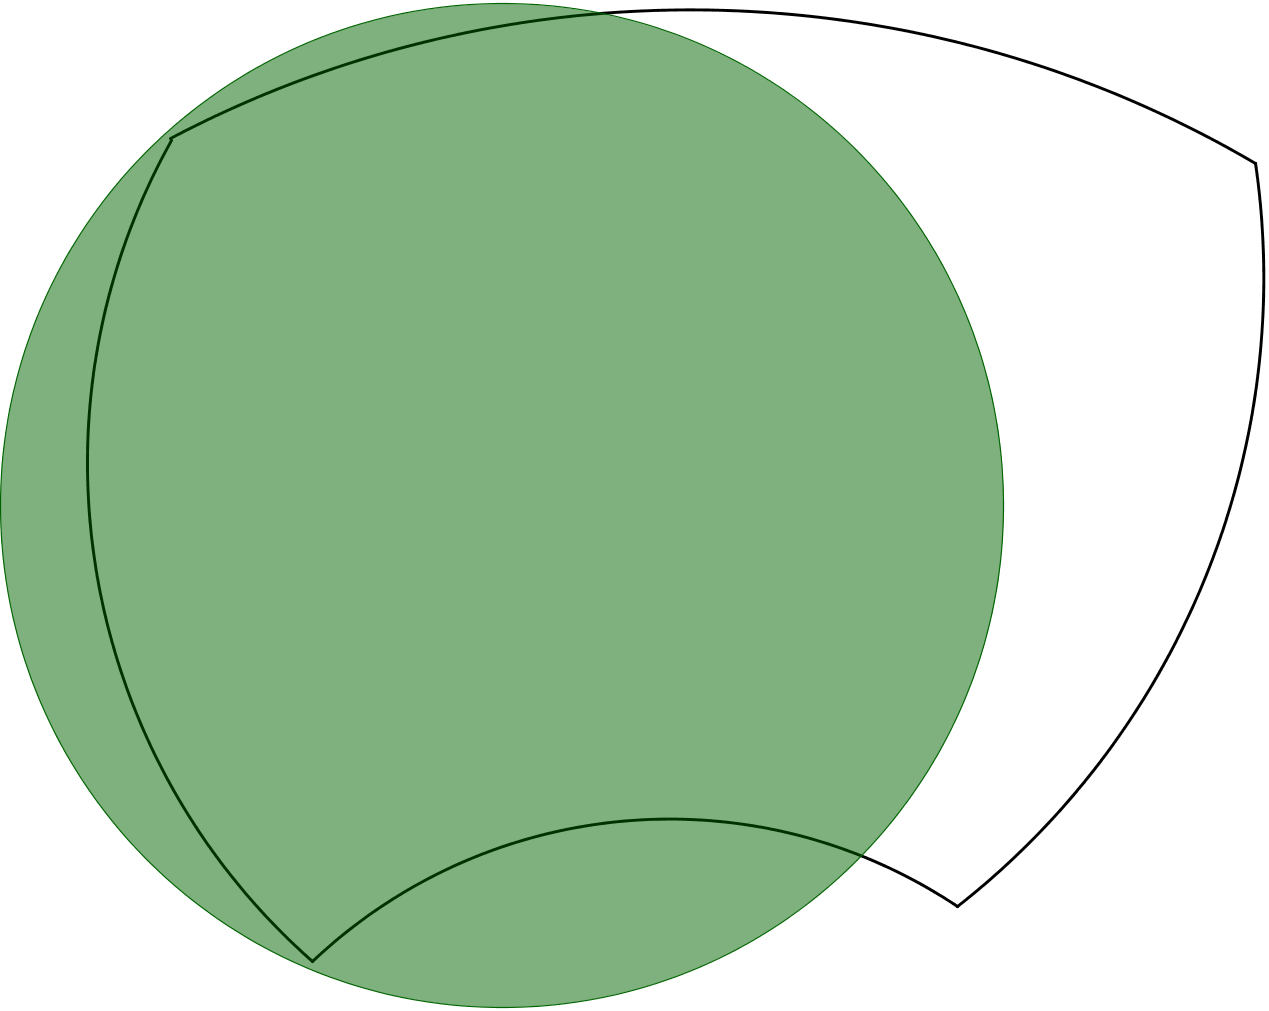
\includegraphics[width=\columnwidth]{figs/dinamica/workspaceGeometrico.png}
	\caption{Área em verde representa a cobertura do revestimento executada pelo
	manipulador, utilizando a abordagem puramente geométrica.}
	\label{fig::wgeo}
\end{figure}

\begin{figure}[h!]	
	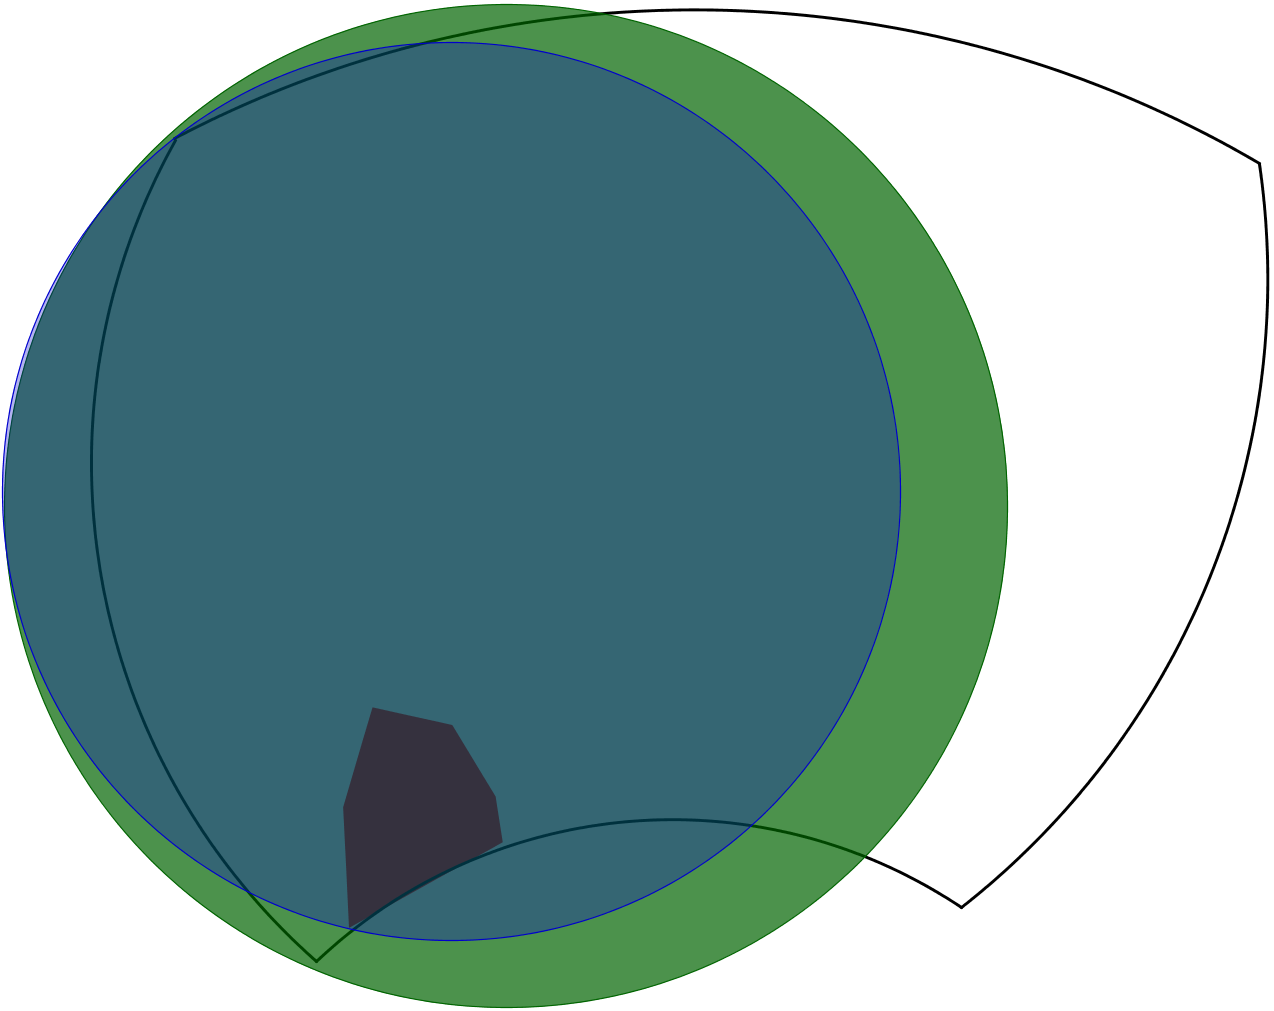
\includegraphics[width=\columnwidth]{figs/dinamica/workspaceCinematica.png}
	\caption{Área em verde representa a cobertura do revestimento executada pelo
	manipulador, utilizando a abordagem puramente cinemática.}
	\label{fig::wcin}
\end{figure}

\begin{figure}[h!]	
	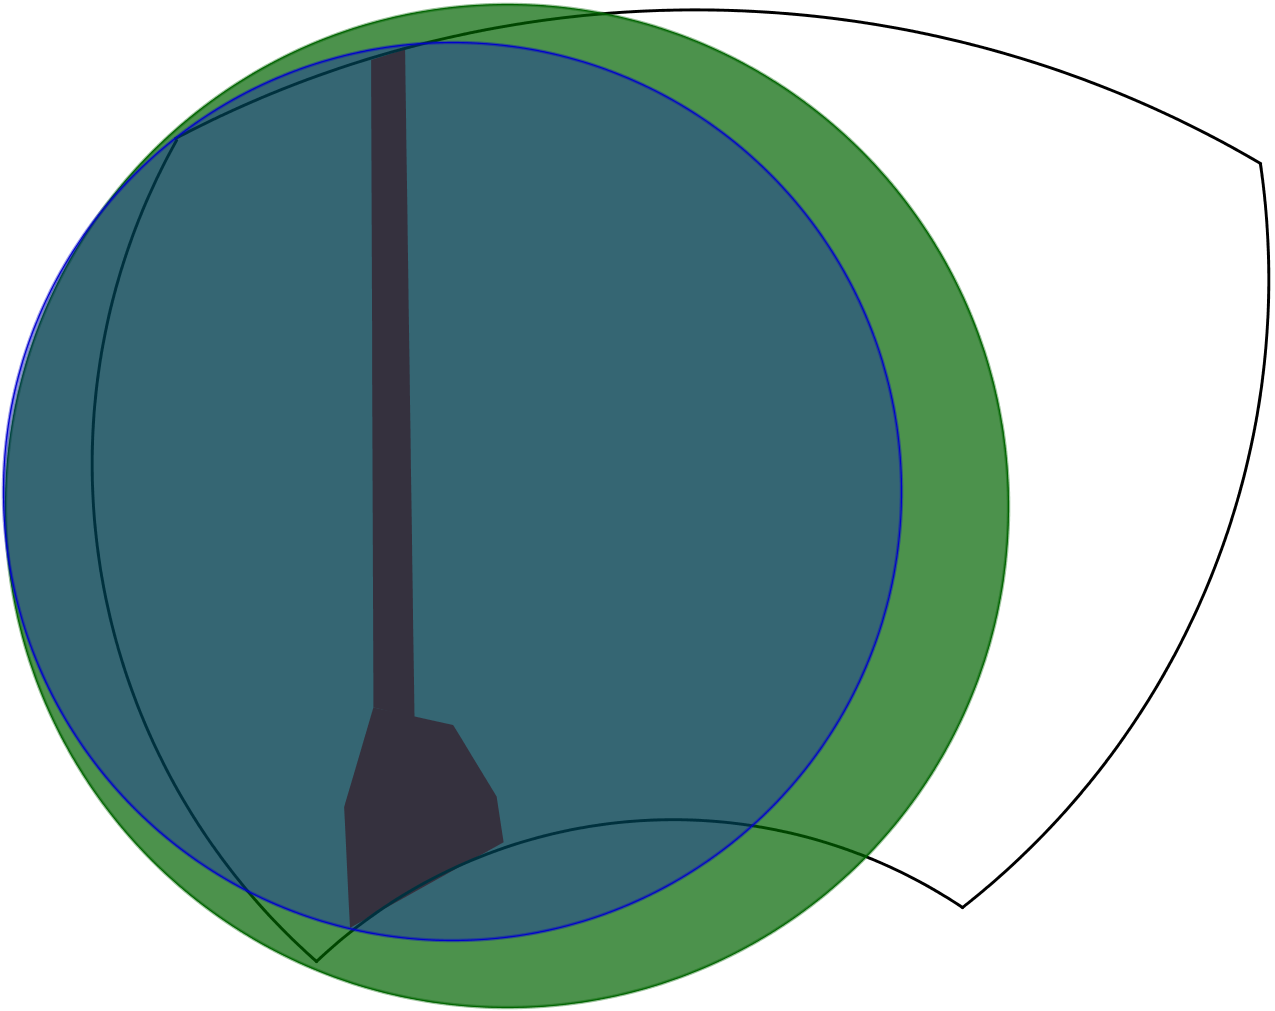
\includegraphics[width=\columnwidth]{figs/dinamica/workspaceTorques.png}
	\caption{Área em verde representa a cobertura do revestimento executada pelo
	manipulador, utilizando a abordagem dinâmica.}
	\label{fig::wdin}
\end{figure}
\subsubsection{Detalhamento da Base Mecânica}\label{sec::base_mec}
A base mecânica é composta pelos elementos de suporte, transporte e ancoragem do
robô no interior da turbina. Os elementos de suporte formam a estrutura
principal da base, que estruturam o ambiente para a montagem, movimentação e
funcionamento seguros do robô. Os elementos de transporte oferecem ao
manipulador graus de liberdade que permitem que este se posicione com facilidade
nos pontos ótimos para o processo. Estes elementos podem ser trilhos, atuadores
lineares, mancais de rolamento, atuadores rotativos, etc. Os elementos de
ancoragem são necessários para fixar o robô e a estrutura no ambiente. As
opções de ancoragem estudadas foram as bases magnéticas e solda, sendo a
primeira opção de preferência pois há menor risco de danificar o ambiente. As
etapas de detalhamento da base mecânica seguem a seguinte ordem: $1)$ investigação dos
graus de liberdade necessários; $2)$ configuração conceitual da base em função
dos graus de liberdade; $3)$ escolha do melhor conceito; $4)$ escolha e
dimensionamento dos elementos mecânicos que compõem a base; $5)$ testes.
Avaliamos até esta etapa do projeto os itens: $1$,$2$ e $3$.

Os graus de liberdade são fornecidos através de combinações de juntas
prismáticas e rotacionais, que no nosso caso irão permitir o movimento do robô
desde a escotilha até o ponto de interesse para o início do processo de
revestimento e entre as etapas de em cada região da pá.
Investigou-se primeiramente alguns conceitos baseados nos graus de liberadade 
necessários para fornecer à base do robô todos os posicionamentos necessários, 
de acordo com os estudos cinemáticos e dinâmicos descritos  nas
seções~\ref{sec::cinematica} e \ref{sec::dinamica}.
%TODO criar label para sec estudo dinamico

A análise dos conceitos estudados permite então compara-los e definir o que
melhor se adapta ao objetivo da solução. Nesta etapa incia-se o detalhamento da base
mecânica seguindo as diretrizes e requisitos mecânicos do projeto. A
estrutura deve ter capacidade de suportar os esforços dinâmicos do robô,
de forma que não haja grandes deformações elásticas e oscilações que possam
comprometer a precisão de posicionamento do efetuador do braço robótico.
Deve-se atentar também ao caráter dinâmico dos esforços, que causam vibrações
que podem resultar em esforços e deslocamentos elevados.
Assim, a fixação da estrutura da base no ambiente deve ser o mais rígida
possível, superdimensionando os elementos de ancoragem e minimizando as folgas
nos acoplamentos.

A entrada dos componentes da base é uma tarefa trabalhosa, devido ao acesso
limitado ao interior da turbina. O diâmetro de $800~mm$ da escotilha inferior
limita o tamanho e geometria dos equipamentos. Além disso, estes componentes devem ser
içados até a escotilha em uma altura de $5~m$ entre o piso no exterior do
ambiente confinado e seu interior. Assim, a modularidade dos elementos que compõe a base
é uma diretriz essencial a esse projeto. A facilidade de transporte, montagem e
desmontagem da base mecânica causará um grande impacto na praticidade e
agilidade de implementação da solução.

A seguir apresenta-se os conceitos analisados, em relação aos graus de
liberdade da base mecânica:

$\bullet$~\textbf{Base Prismática-Rotacional-Rotacional (P-R-R):}
  
  Neste conceito estudou-se a possibilidade de utilizar uma base com $3$ graus
  de liberdade: um prismático e dois rotacionais. O prismático seria composto
  por um trilho alinhado e paralelo ao eixo da turbina que transportaria o robô
  até a região próxima a pá. Uma junta rotacional e com eixo vertical orientaria
  a base nesta direção e uma junta perpedincular à primeira faria o
  posicionamento da base do robô para então iniciar o processo de revestimento.
  A figura~\ref{fig::base_prr} ilustra este conceito.
    
  \begin{figure}[h!]
   \centering
   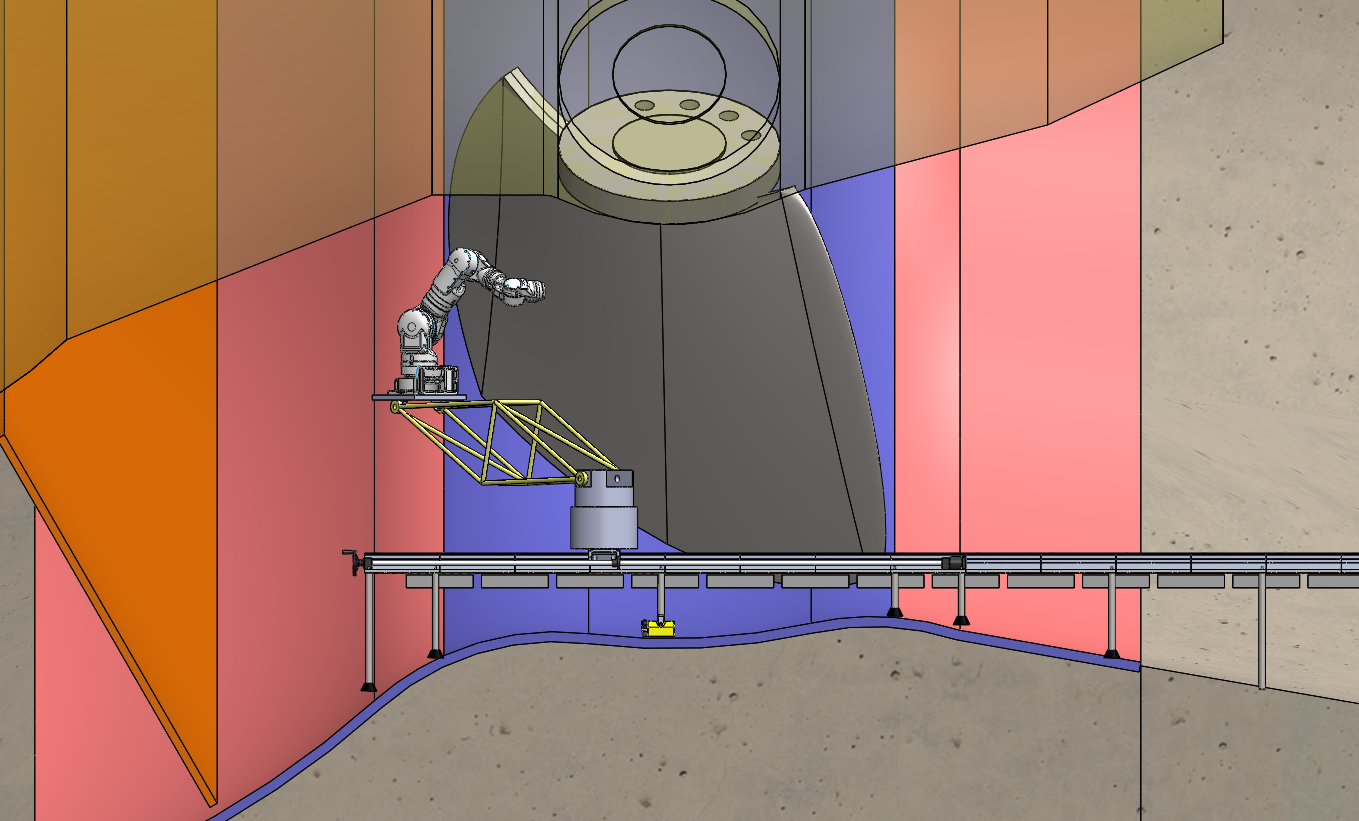
\includegraphics[width=0.8\columnwidth]{figs/bases/base_prr}
   \caption{Base Primático-Rotacional-Rotacional}
   \label{fig::base_prr}
\end{figure}

  A vantagem deste conceito é conferir um alcance grande ao manipulador através
  da base, permitindo que este possa ser de menor alcance próprio, mas ao mesmo
  tempo mais leve.
  Porém, devido à configuração de juntas e pelos resultados encontrados no
  estudo cinemático, a manobrabilidade desta base seria reduzida naquele espaço,
  havendo posicionamentos difíceis de serem alcançados, ou até impossíveis
  dependendo do manipulador escolhido.
  
$\bullet$~\textbf{Base Prismática (P):}

  Este conceito consiste de um trilho (junta prismática) para o transporte do
  manipulador desde a escotilha até o ponto de interesse para revestimento na
  face anterior ou posterior da pá. Quando posicionado, remove-se a seção
  do trilho na direção que obstrui a rotação do rotor. Neste conceito,
  adiciona-se um grau de liberdade ao sistema utilizando a própria rotação do
  rotor, posicionando a pá em relação ao robô. A base mecânica então forneceria
  apenas movimento no trilho na direção do eixo da turbina, deixando fixas as
  outras direções. O procedimento para o revestimento seria o posicionamento do
  rotor, deixando a região a ser processada ao alcance do manipulador; o
  posicionamento do robô no trilho, em relação a pá; a ancoragem do robô
  no ambiente; e o revestimento da região possível para aquela posição.
  Repete-se então este procedimento até ter toda a face processada e
  posiciona-se a próxima pá para revestimento, sem necessidade de mover ou
  desmontar a base do robô até todas as faces daquele lado estarem completas.  A
  figura~\ref{fig::base_p} ilustra este conceito.
  
  \begin{figure}[h!]
   \centering
   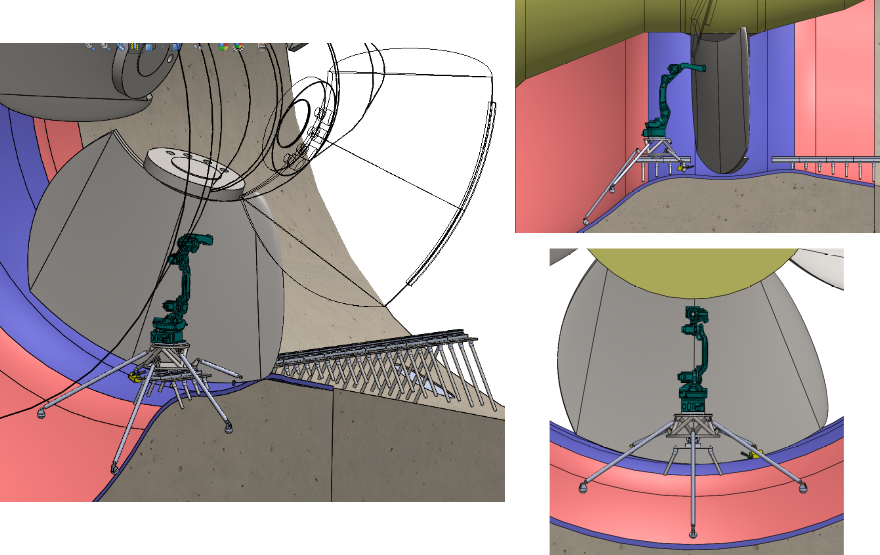
\includegraphics[width=0.8\columnwidth]{figs/bases/base_p}
   \caption{Base Prismática}
   \label{fig::base_p}
\end{figure}
  
  Este conceito foi estudado para o manipulador MH$12$, que de acordo com a
  análise cinemática consegue processar toda a extensão vertical. Para outros
  manipuladores, seria necessário incluir uma junta prismática, adicionando um
  grau de liberdade, na direção vertical.
  
  A análise cinemática também demonstrou que seriam necessárias muitas posições
  do rotor para completar uma face da pá. Há inclusive dificuldades operacionais e
  de segurança no procedimento de rotação do rotor que devem ser considerados. O
  rotor só pode ser girado manualmente, não fornecendo precisão no
  posicionamento da pá em relação a base. Por ser uma tarefa manual, deve-se ter
  procedimentos adequados de segurança para preservar tanto o operador quanto os
  equipamentos próximos. Estas preocupações tornam a solução pouco prática sob o
  ponto de vista operacional.

$\bullet$~\textbf{Base Prismática-Rotacional-Prismática (P-R-P):}

  Este conceito consiste de uma base composta por um trilho primário (junta
  prismática $1$), uma plataforma de base pivotada por mancal e rolamentos entre
  o trilho primário e secundário (junta rotacional) e um trilho secundário
  (junta prismática $2$). Montado o trilho primário alinhado ao eixo da turbina
  a base rotacional sobre o trilho primário, fixa-se o robo sobre a base
  rotacional. Esta base permitrá a montagem do trilho secundário apenas quando o
  robô atingir a região de interesse para revestimento. Quando posicionado o
  manipulador, monta-se então o trilho secundário alinhado ao plano paralelo a
  face da pá e ancora-se a base no ambiente. Desta forma, o robô pode-se
  movimentar ao longo de toda a extensão da pá por meio do trilho secundário e
  também se aproximar e se afastar da superfície da pá, por meio do trilho
  primário. A figura~\ref{fig::base_prp} ilustra este conceito.

\begin{figure}[h!]
   \centering
   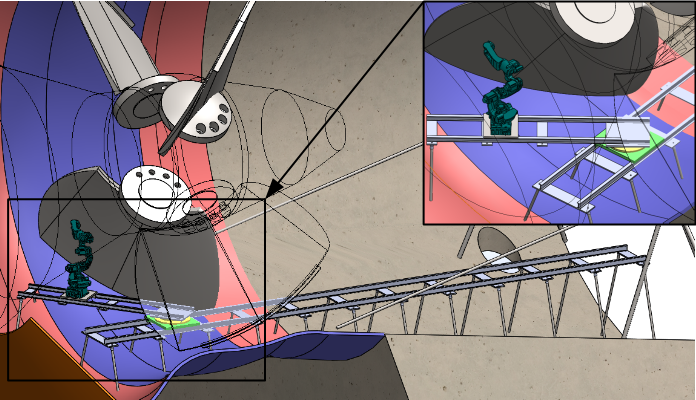
\includegraphics[width=0.9\columnwidth]{figs/bases/base_prp}
   \caption{Base Primática-Rotacional-Prismática}
   \label{fig::base_prp}
\end{figure}

  Desta forma, o rotor deve estar girado em, no mínimo $30^o$ para não haver
  contato com o trilho primário. A análise cinemática será realizada para
  encontrar a melhor configuração de juntas da base que permite ao robô se
  movimentar nos graus de liberdade da base, sem alterar o posicionamento do
  rotor e, assim, cobrir uma face inteira da pá. Para a repetição do processo
  nas outras pás do lado da sucção da turbina, é necessária a desmontagem do
  trilho secundário, o recuo do robô e desmontagem de parte do trilho primário,
  permitindo o giro do rotor para a pá seguinte.
  Para as faces do lado de adução, não é necessária a desmontagem parcial do
  trilho primário.
  
\subsubsection{Sistemas de elevação, fixação e ancoragem}
A entrada de pessoal através da escotilha é feita por uma escada vertical com
guarda-corpo com uma altura total de $5~m$. Equipamentos de segurança como
cinto e talabarte devem ser usados para qualquer um que deseja entrar no
ambiente confinado da turbina, através da escada e isso impossibilita o
transporte manual dos equipamentos. Por este motivo, deve ser instalada uma
estrutura com talha que permita a elevação até o interior da turbina e
movimentação para a áera de montagem adequada. As figuras~\ref{fig::talha} e
\ref{fig::talha_trilho} ilustram a estrutura de elevação com talha e carro
trole. 
  
\begin{figure}[h!]
   \centering
   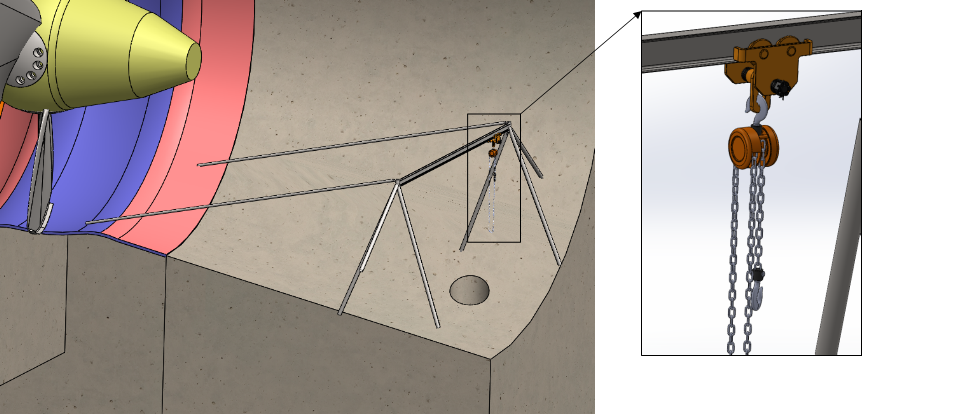
\includegraphics[width=0.8\columnwidth]{figs/bases/talha}
   \caption{Sistema de elevação dos equipamentos}
   \label{fig::talha}
\end{figure}

\begin{figure}[h!]
   \centering
   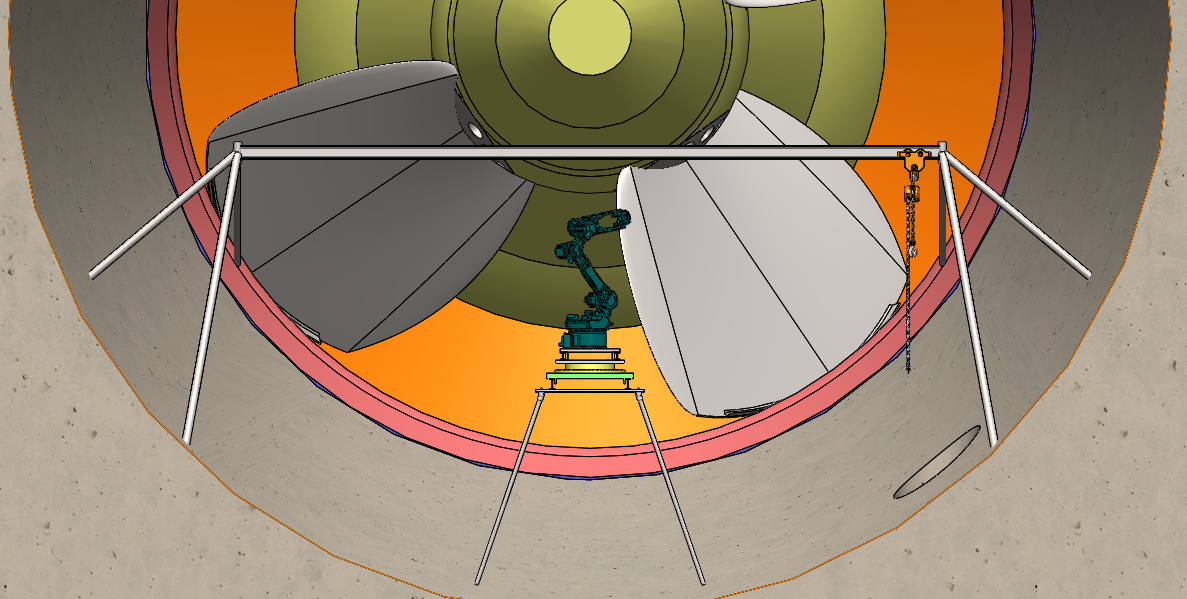
\includegraphics[width=0.8\columnwidth]{figs/bases/talha_trilho}
   \caption{Visão frontal da talha e trilho}
   \label{fig::talha_trilho}
\end{figure}

Devido aos esforços dinâmicos de operação do robô, a fixação da estutura da
base mecânica no ambiente deve ser dimensionada com cuidado. Por se
tratar de um ambiente de escoamento de fluido sob pressão, não são admitidas
modificações permanentes de infra-estrutura no interior da turbina, logo,
qualquer método de fixação utlizado deve ser removível, sem causar nenhum dano
à qualquer superfície. Em visita técnica realizada em Outrubro de $2015$ foi
testada a viabilidade de utlização de bases magnéticas para o sistema de
ancoragem e fixação. Este teste teve o objetivo de verificar a real carga limite de tração
do imã, considerando o ambiente (geometria), materiais e acabamentos
superficiais reais a que estará submetido na solução final. O resultado
detalhado do teste encontra-se no Apêndice~\ref{ape::magnetic}.

Outra opção para fixação provisória seria a soldagem da estrutura na
superfície do túnel. Esta opção segue como uma alternativa ainda para regiões
de difícil fixação da base magnética.
  
\subsubsection{Shutter}%TODO mudar o nome do sistema de desvio do fluxo de
% revestimento
O processo de revestimento HVOF (\textit{High Velocity Oxygen Fuel}) requer
velocidade da pistola controlada de $40~m/min$. Esta velocidade é essencial para
a qualidade do processo e deve ser mantida constante para se obter uma camada 
regular de material ao longo de toda a superfície da peça. Na solução
pesquisada demonstou-se ser inviável utilizar um robô de grande porte, devido a
limitação de acesso e ao confinamento do manipulador no ambiente. Portanto, o
manipulador  escolhido realizará o processo em regiões delimitadas da
superfície da peça e na trajetória haverá inevitavelmente mudanças de direção e
portanto acelerações que irão variar a velocidade da pistola. Durante essas
variações não deve-se injetar o material na peça, sendo necessário um mecanismo
autônomo para impedir o processo nestes intervalos.

A ideia inicialmente estudada foi de uma barreira ao fluxo na saída da pistola. 
A figura~\ref{fig::shutter_todos} ilustra a ideia para dois conceitos nas
configurações aberta e fechada. 
Nestes conceitos, uma barreira é movimentada automaticamente sempre que houver
mudança de direção da pistola, impedindo que o fluxo de material atinja a
pistola. 

\begin{figure}[h!]
   \centering
   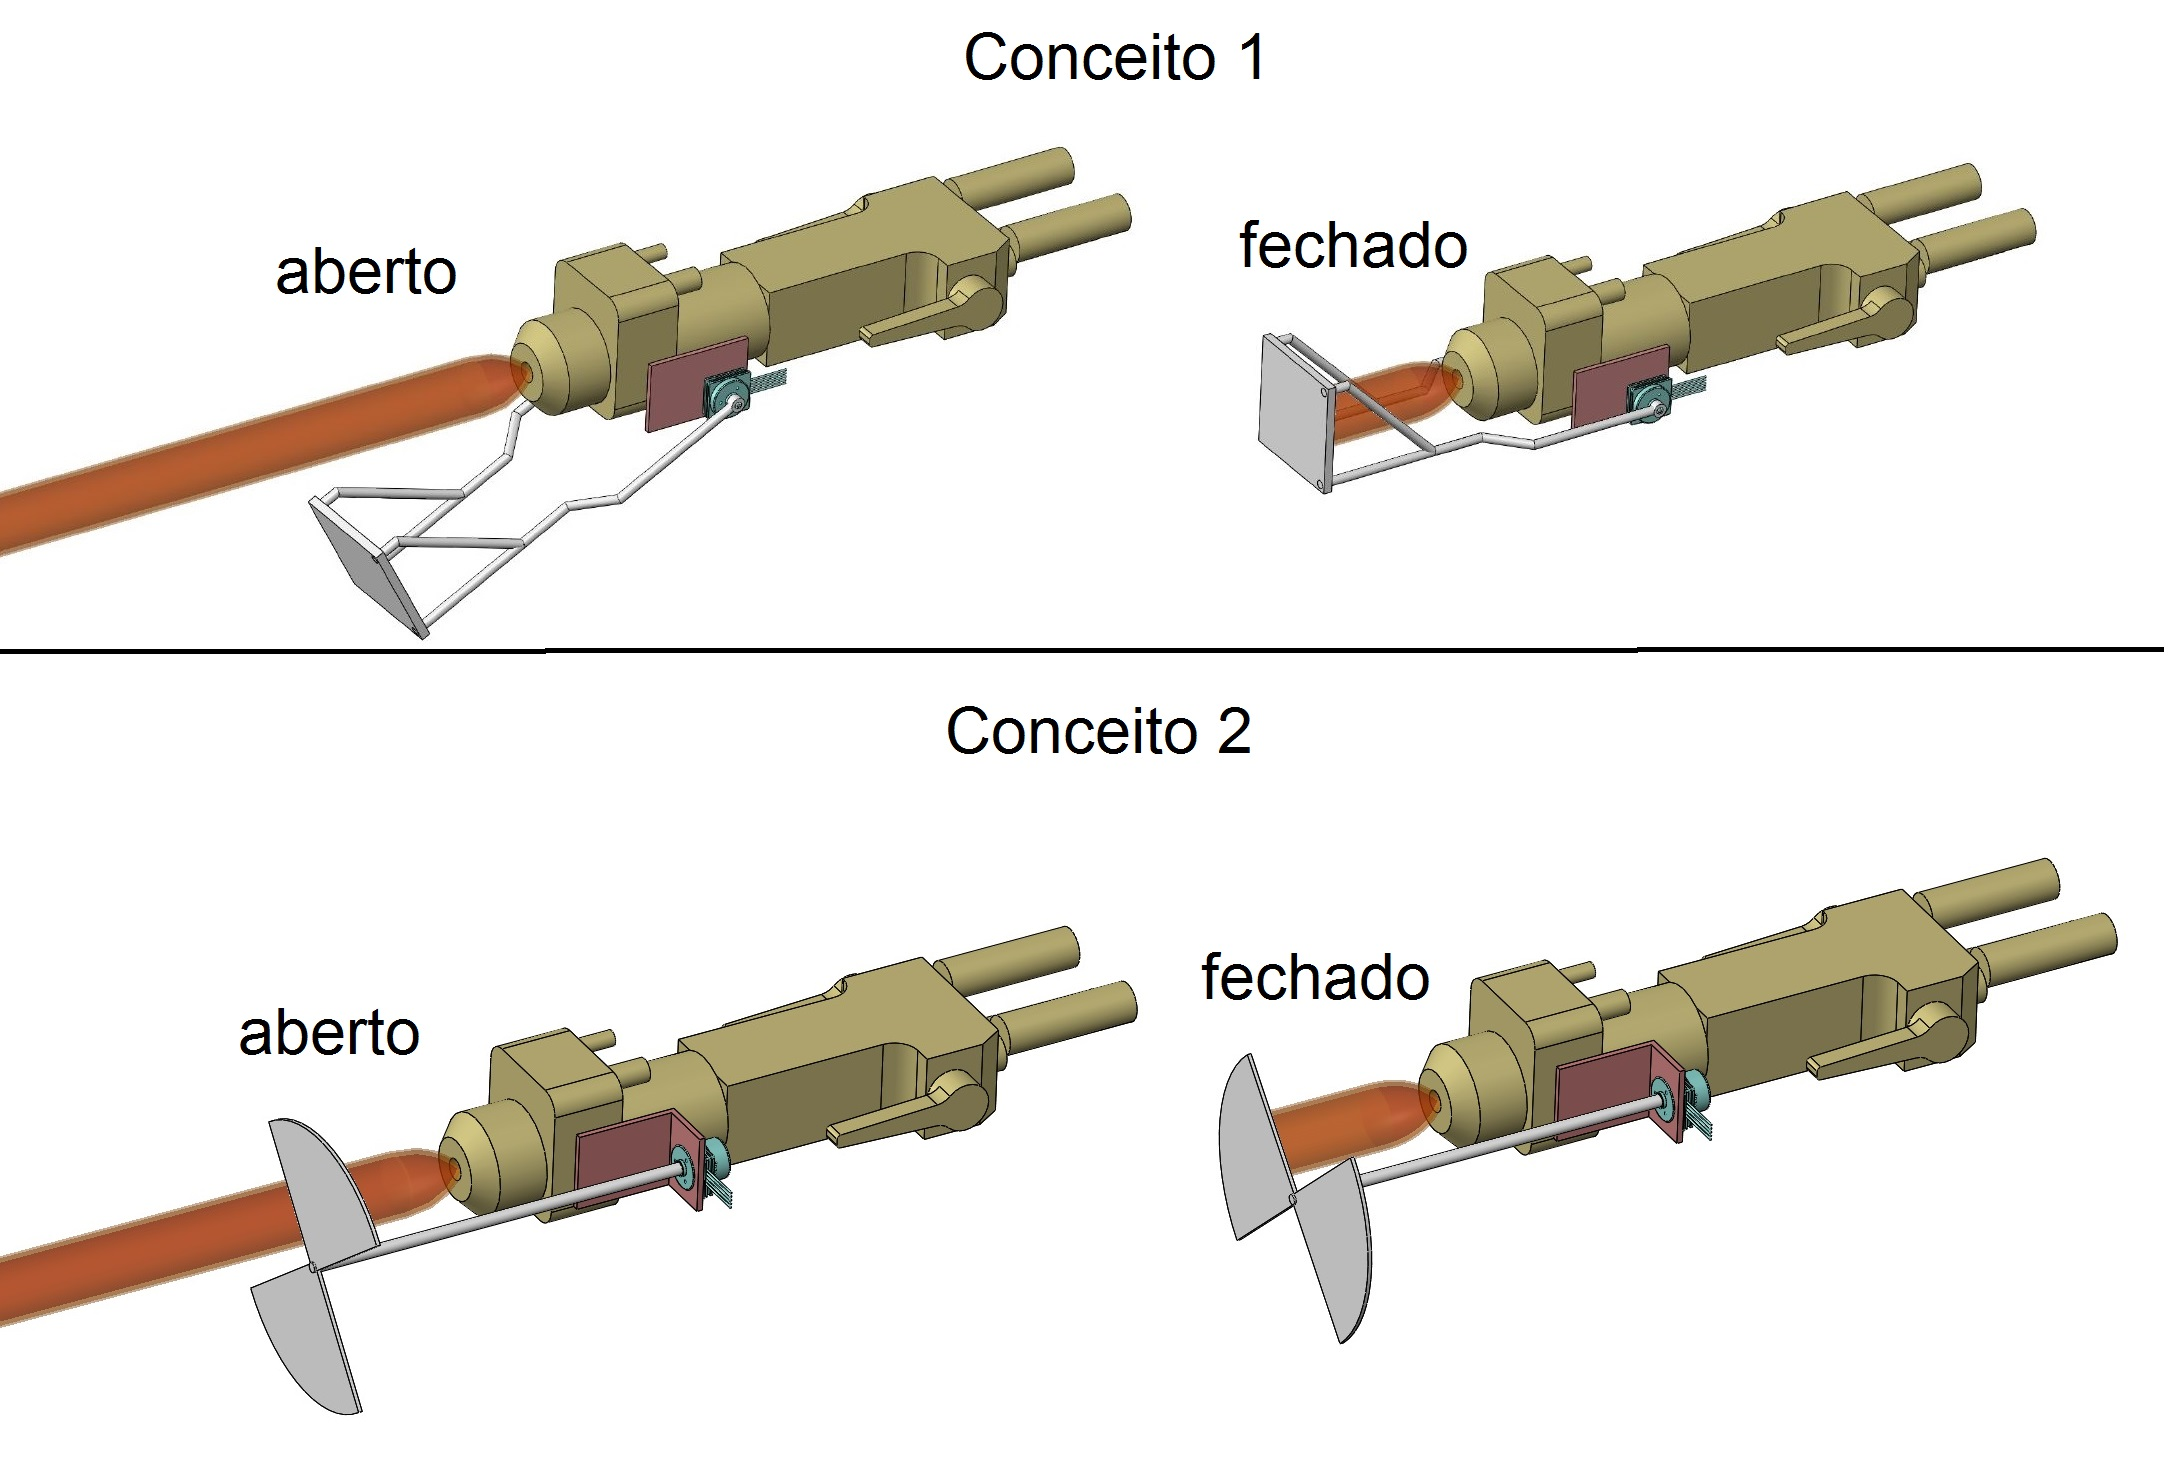
\includegraphics[width=0.8\columnwidth]{figs/shutter/shutter_todos}
   \caption{Conceitos de Shutter avaliados}
   \label{fig::shutter_todos}
\end{figure}

Algumas considerações foram levantadas para avaliar a viabilidade
desta solução, como a alta temperatura da chama, a capacidade do atuador, a
resistência mecânica da barreira e a taxa de acúmulo de material. Este conceito
foi abandonado principalmente devido ao acúmulo de material na barreira, o que
levaria a um aumento de seu peso e por consequência momento de inércia,
alterando a dinâmica prevista ou ainda poderia chegar a obstruir a saída da
chama, causando danos à pistola.

Outra proposta que está sendo estudada é a de modificar o fluxo da linha de
revestimento. A ideia é a inclusão de uma válvula direcional com atuação por
solenóide para desviar o fluxo do material de revestimento para um tanque ou
cilindro de retorno. Esta atuação deve ser autônoma assim como a
trajetória do manipulador. A válvula seria de três vias e duas posições ($3/2$) tal que, no 
repouso, direciona-se o fluxo diretamente para a pistola e, quando
atuada, bloqueia-se o fluxo para a pistola e abre-se o fluxo para exaustão. Uma
válvula limitadora de pressão regulável seria utilizada na linha de exaustão
para igualar as diferenças de pressão entre as duas vias, minimizando efeitos transitórios.
A figura~\ref{fig::circuito_hvof} apresenta o circuito do processo HVOF de forma
simplificada.

 \begin{figure}[h!]
   \centering
   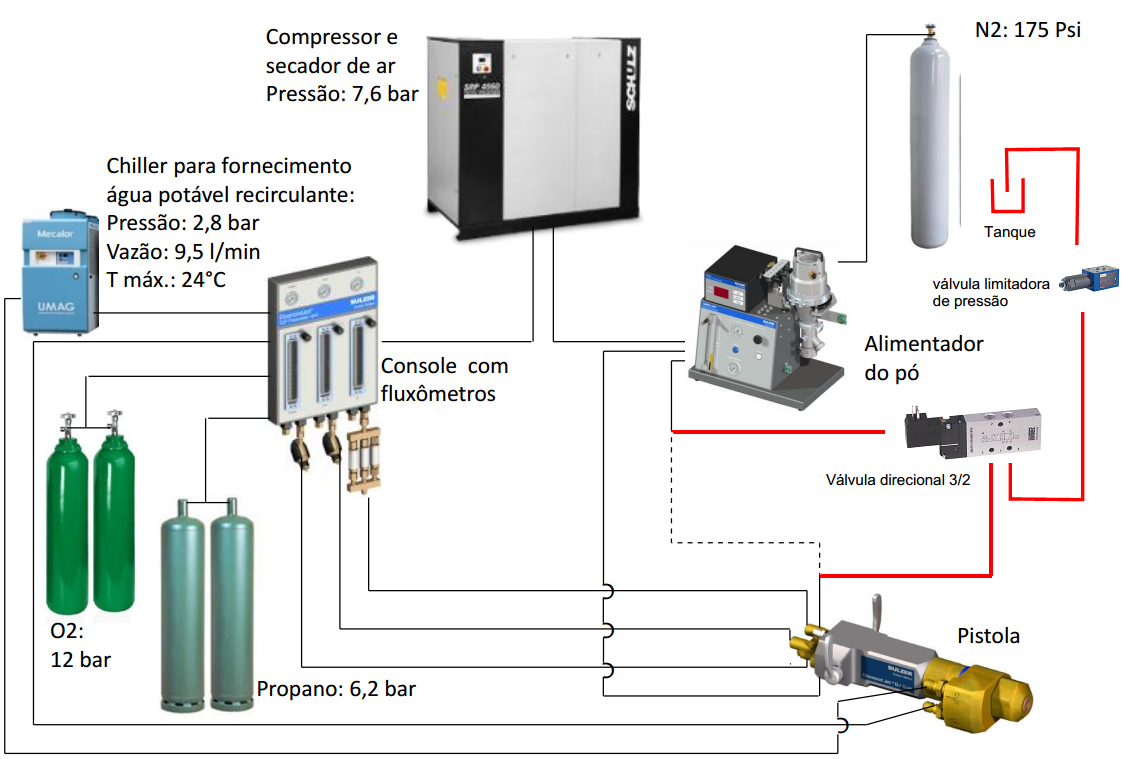
\includegraphics[width=0.8\columnwidth]{figs/shutter/Circuito_HVOF_mod}
   \caption{Circuito do processo HVOF modificado}
   \label{fig::circuito_hvof}
\end{figure}

A linha tracejada representa o circuito original, as linhas em vermelho
representam a modificação do circuito com os equipamentos adicionais indicados.

Esta é uma alternativa que tem como principal vantagem a de poder retornar a
matéria-prima do revestimento para tanque, ou seja, evita-se
o desperdício do material no ambiente. Esta matéria-prima poderia então ser
reaproveitada no processo, separando-se o gás.
 
\section{Localização}\label{sec::localizacao}

\subsection{Estudo de sensores 3D}

O processo de metalização utilizado atualmente considera que a posição e
orientação da pá é fixa em relação ao robô e, uma vez, que corretamente
posiciona, o processo é executado em malha aberta. Entretanto, para qualquer uma
das soluções propostas por esse documento, não é possível assumir que nem a
posição nem a orientação do manipulador, em relação a pá a ser processada, se
manterão fixas.

Para um correto planejamento de trajetória que o manipulador deve seguir durante
a tarefa de metalização, é importante o conhecimento da transformada entre o
sistema de coordenada do manipulador e da pá a ser processada. Portanto, é
necessário utilizar algum sistema que possibilite a aquisição de informações a
respeito do ambiente e da posição relativa entre o manipulador e as pás.

A utilização de um sensor de aquisição de dados espaciais não se limita somente
a localização, mas, dependendo do sistema a ser escolhido, pode também ser útil
na reconstrução do modelo do perfil hidráulico da pá, tanto do perfil ideal
quanto do estado atual da pá a ser processada (Tarefas descritas em
\ref{sec::introducao}).

Esta seção irá apresentar os segmentos de sensores capazes de suprir essa
necessidade, assim como suas vantagens e limitações. 


\subsubsection{3D scanners}

3D scanners são equipamentos de alta precisão utilizados na indústria
geralmente em aplicações de metrologia, construção civil, monitoramento de
deformações, entre outras. O equipamento consiste em um feixe de laser que é
direcionado por meio de um espelho e a partir da mudança de fase do sinal
refletido é possível calcular a distância até o objeto atingido.

\paragraph{FARO Focus3D X330}

\begin{itemize}
  \item Campo de visão (vertical/horizontal): $300^o$ / $360^o$
  \item Tamanho do passo (vertical/horizontal): $0,009^o$ (40.960 3D-Pixel em
  $360^o$)
  \item Velocidade máx. de varredura vertical: 5.820 rpm ou 97 Hz
  \item Precisão: $\pm$2mm
  \item Peso: 5,2 kg
  \item Tamanho: 240 x 200 x 100 mm
  \item Vida da bateria: 4,5 horas
  \item Temperatura ambiente: $5^o$ - $40^o$ C
\end{itemize}
%TODO LEMBERAR QUE EXISTE LASER TRIANGULATION TAMBÉM!

\paragraph{Velodyne}

A empresa Velodyne possui, atualmente, 3 modelos de 3D Lidar. Os modelos variam
basicamente no número de pares de emissores e receptores e, consequentemente, na
resolução final. Os modelos são o VLP-15, o HDL-32E e HDL-64E, com 16,32 e 64
canais respectivamente. O modelo mais utilizado é o intermediário HDL-32E, que
tem um preço na faixa de U\$30k.

\begin{itemize}
\item 32 pares laser/detector  
\item Campo de Visão: +10.67$^o$ to -30.67$^o$ (vertical)
\item Rotação de $360^o$
\item Alcance - 1m - 100m 
\item 10 Hz frame rate (selecionável 5-20Hz)
\item Temperatura de Operação $-10^o$ to $+60^o$ C
\item Acurácia: $<$2 cm
\item Resolução Angular (vertical) 1.33$^o$
\item Peso: HDL-32E = 1kg; Cabos = 0.3kg
\item Tamanho: 15cm altura x 8.6cm diâmetro
\item Proteção: IP67
\item Correção de orientação (internal MEMS acelerometros and gyros)
\end{itemize}

\begin{figure}[h!]
   \centering
   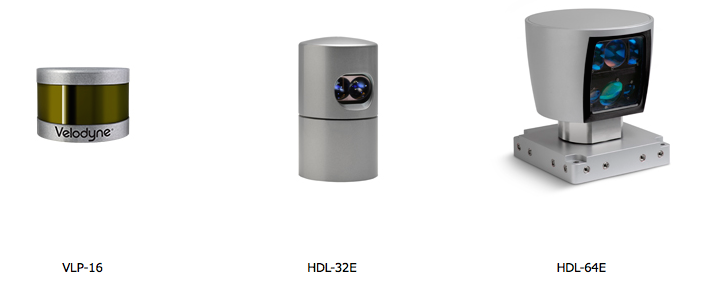
\includegraphics[width=0.8\columnwidth]{figs/3dsensors/velodyne}
   \caption{Velodyne Models}
   \label{fig::velodyne_models}
\end{figure}

\paragraph{Forecast 3D Laser System}


O sensor Forecast 3D consiste em um senor 2D laser da SICK, modelo LMS 151 ou
511, acoplado a uma unidade $pan-tilt$. O seu preço esta na faixa de U\$37k.


\begin{figure}[h!]
   \centering
   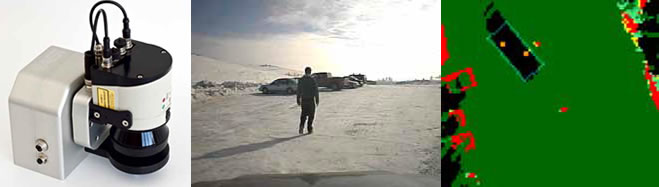
\includegraphics[width=0.8\columnwidth]{figs/3dsensors/forecast}
   \caption{Forecast 3D Laser System}
   \label{fig::forecast}
\end{figure}

%TODO exemplos dos sensores de 3D scanners
%TODO Pros e cons

\subsubsection{ToF Cameras}

As conhecidas como Time-of-Flight são dispositivos compostos por apenas uma
câmera, não necessitando de uma configuração stereo para triangularização de
imagens. Esse tipo de dispositivo utiliza uma fonte infra-vermelho interna e de
forma análoga aos dispositivos laser, calcula a distância a partir da diferença
de fase do sinal refletido. Entretanto, essa tecnologia possibilita o cálculo
simultâneo das distâncias de cada objeto na região iluminada pela fonte IR,
mesmo que com resoluções limitadas.


\paragraph{Sentis M100 / Argos 3D - P100}

\begin{itemize}
  \item Medidas de distância e vídeo em tons de cinza
  \item Resolução: 160 x 120 pixels
  \item 40 - 160 fps
  \item Alcance: $>$3m  (extensível até 10m indoor)
  \item Campo de Visão: $90^o$
  \item Tamanho: 75 x 57 x 26 mm
  \item Peso:
\end{itemize}

\begin{figure}[h!]
   \centering
   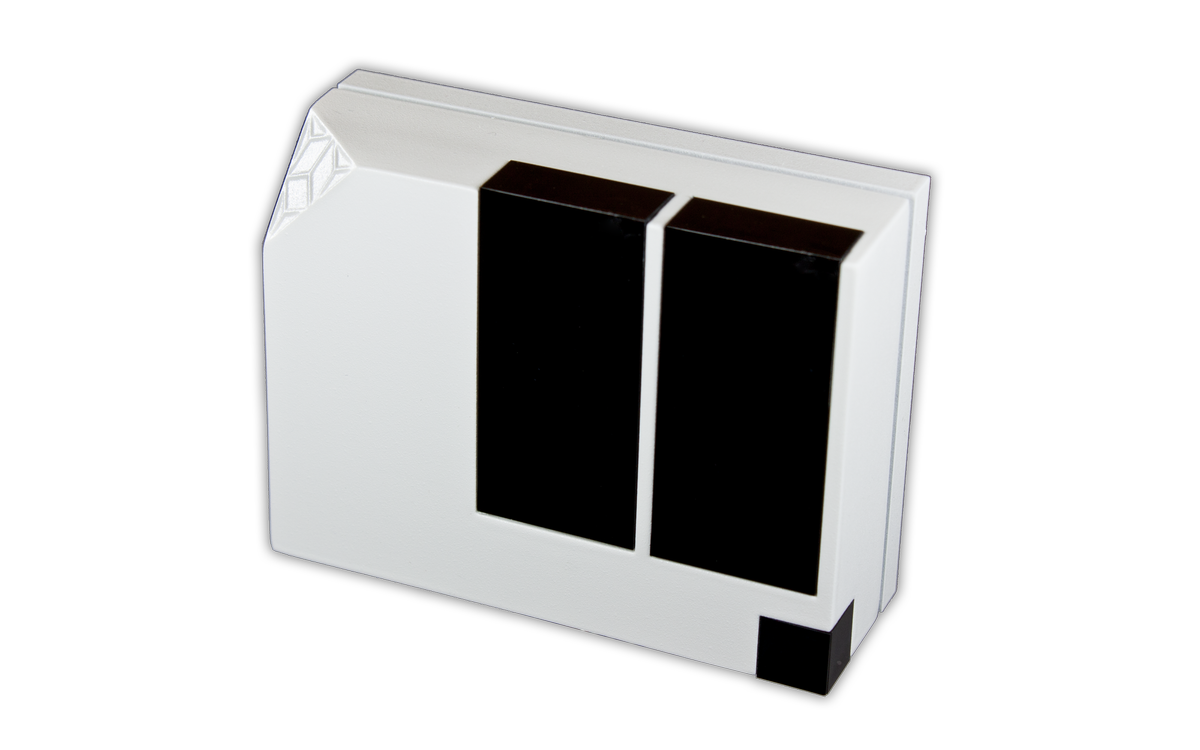
\includegraphics[width=0.8\columnwidth]{figs/3dsensors/argos3dp100}
   \caption{Sensor Argos 3D - P100}
   \label{fig::forecast}
\end{figure}


\subsection{Mesa Imaging SwissRanger SR4000}


\begin{itemize}
  \item Alcance para detecção: 0.1 - 10.0 m
  \item Alcance calibrado: 0.8 - 8.0 m
  \item Drift com a temperatura (T) - $\leq$ 1.5 mm/$^o$C (max.) - For 10$^o$C
  $\leq$ T $\leq$ 50$^o$C
  \item Tamanho: 65 x 65 x 76 mm
  \item Peso: 510 g
\end{itemize}

\begin{figure}[h!]
   \centering
   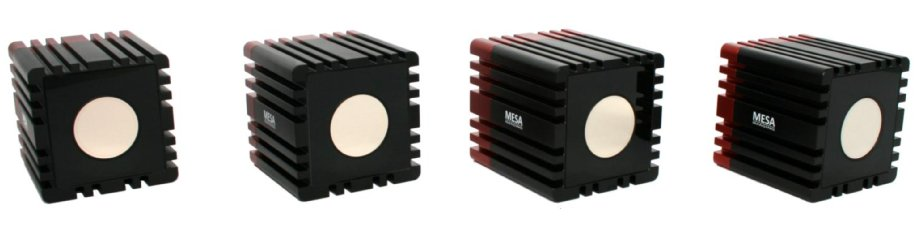
\includegraphics[width=0.8\columnwidth]{figs/3dsensors/mesa2}
   \caption{Mesa Imaging SwissRanger SR4000}
   \label{fig::mesa}
\end{figure}
%TODO exemplos dos sensores de ToF

Essa tecnologia tem como vantagem o tamanho relativamente compacto dos sensores,
não precisa de calibração extrínseca e também não é muito sensivel a iluminação
presente no ambiente, pois possui fonte de iluminação própria.

%TODO Pros e cons

\subsubsection{Câmeras de Luz Estruturada}

Estes sensores constituem de uma fonte emissora de infra-vermelho e um receptor.
Um padrão é projetado na cena a ser reconstruida e a partir da distorção desse
padrão é possível o cálculo de distâncias. 

%TODO exemplos dos sensores de luz estruturada
%TODO Pros e cons

%TODO ELAEL - decidir se abre uma subseção d eaplicações ou coloca um exemplo de
% aplicação em cada componente - utilizar o seu material do SOTA em 3D sensors. 






\section{Conclusão e trabalhos futuros}\label{sec:conclusions}

%TODO concluir os resultados obtidos
%\appendix \section{Pesquisa de mercado}
Nas tabelas, estão marcadas em vermelho as características que os manipuladores
não preencheram, em relação aos requisitos do processo HVOF ou às restrições do
ambiente e logística, de acordo com o acesso em estudo. Em amarelo, são
assinalados os manipuladores que cumpriram com as principais caracterísiticas,
mas ainda não cumprem as exigências da solução conceitual, sendo necessária
alguma alteração no manipulador. Em verde, são assinalados os manipuladores que
cumprem todas as exigências e estão pronto para o uso.
 
\subsection{Acesso pela escotilha inferior - estudo de
mercado}\label{ape::bighatch}
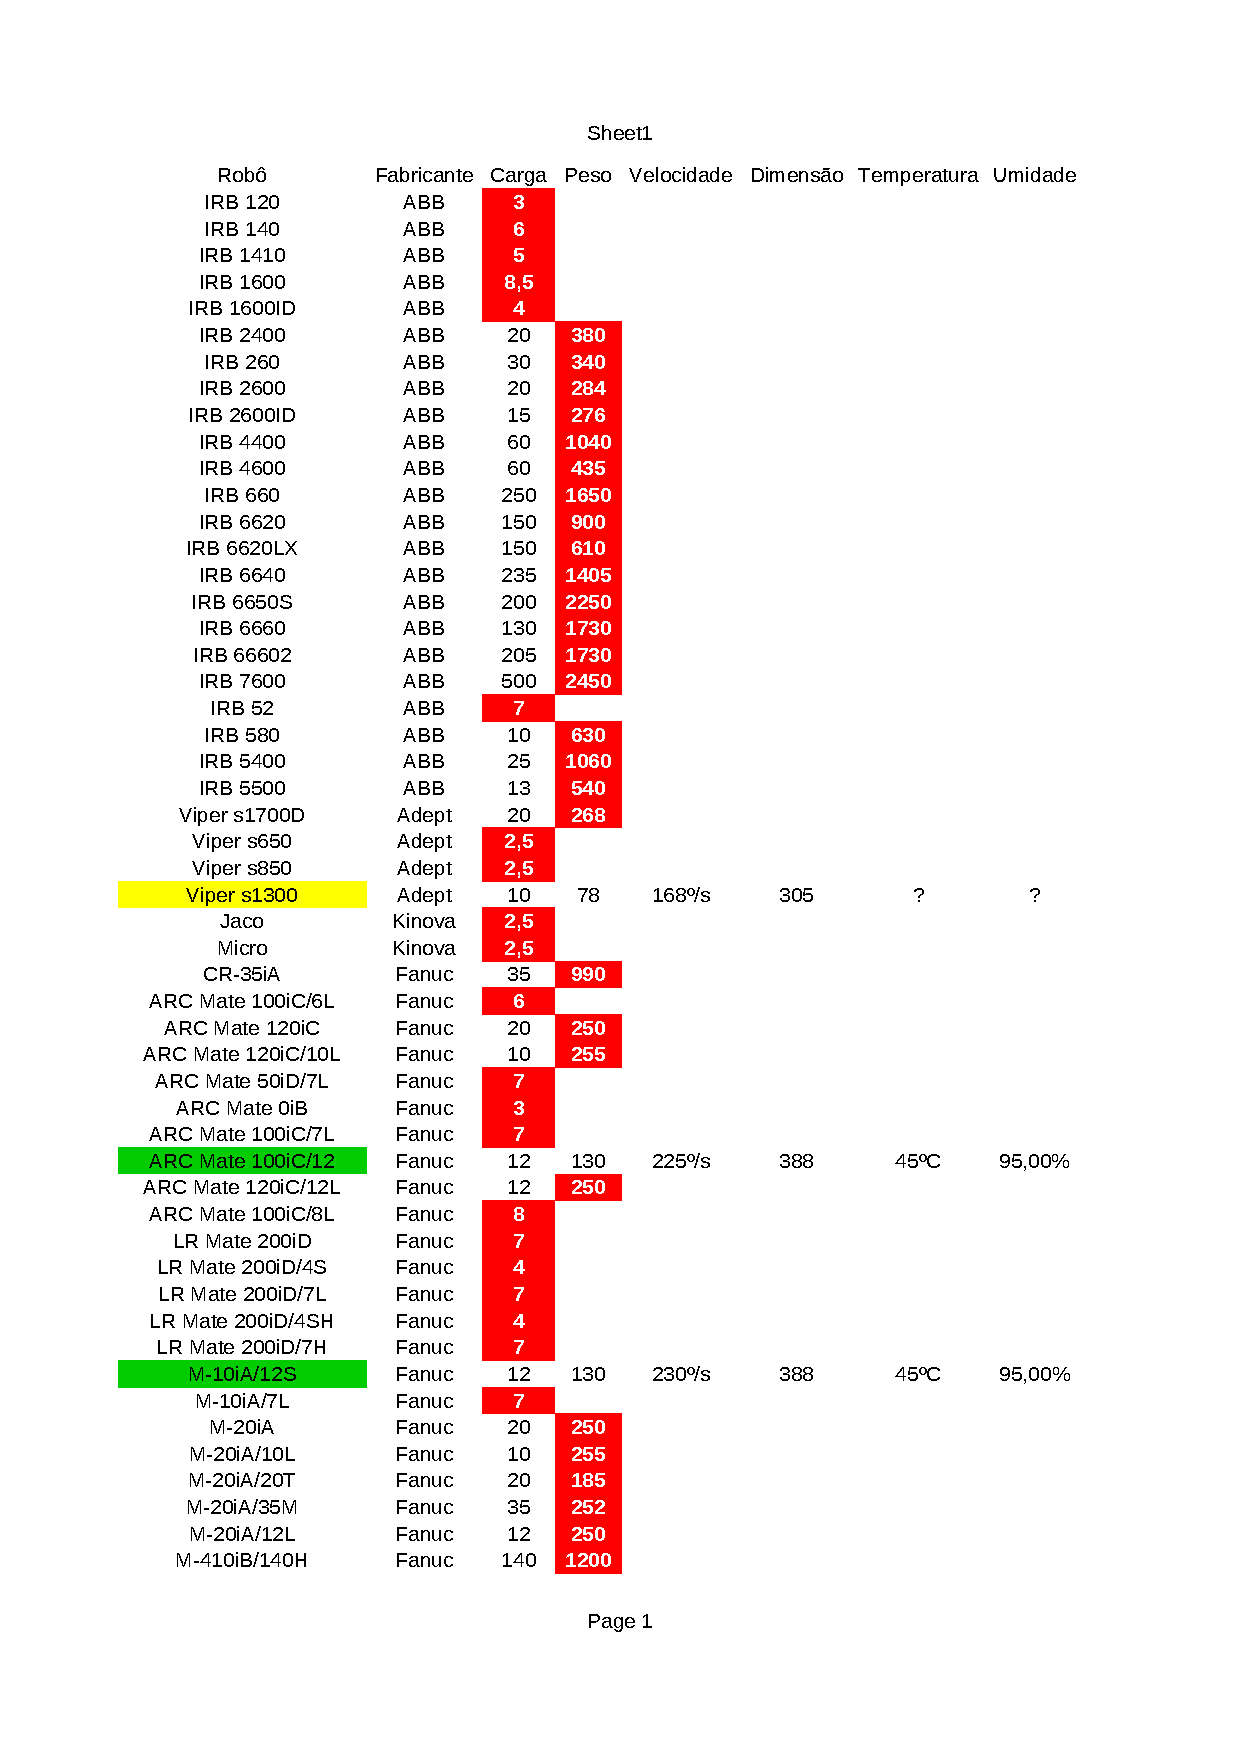
\includepdf[pages=1-]{Apendice/marketbighatch}

\section{Relatório de teste da base magnética}

%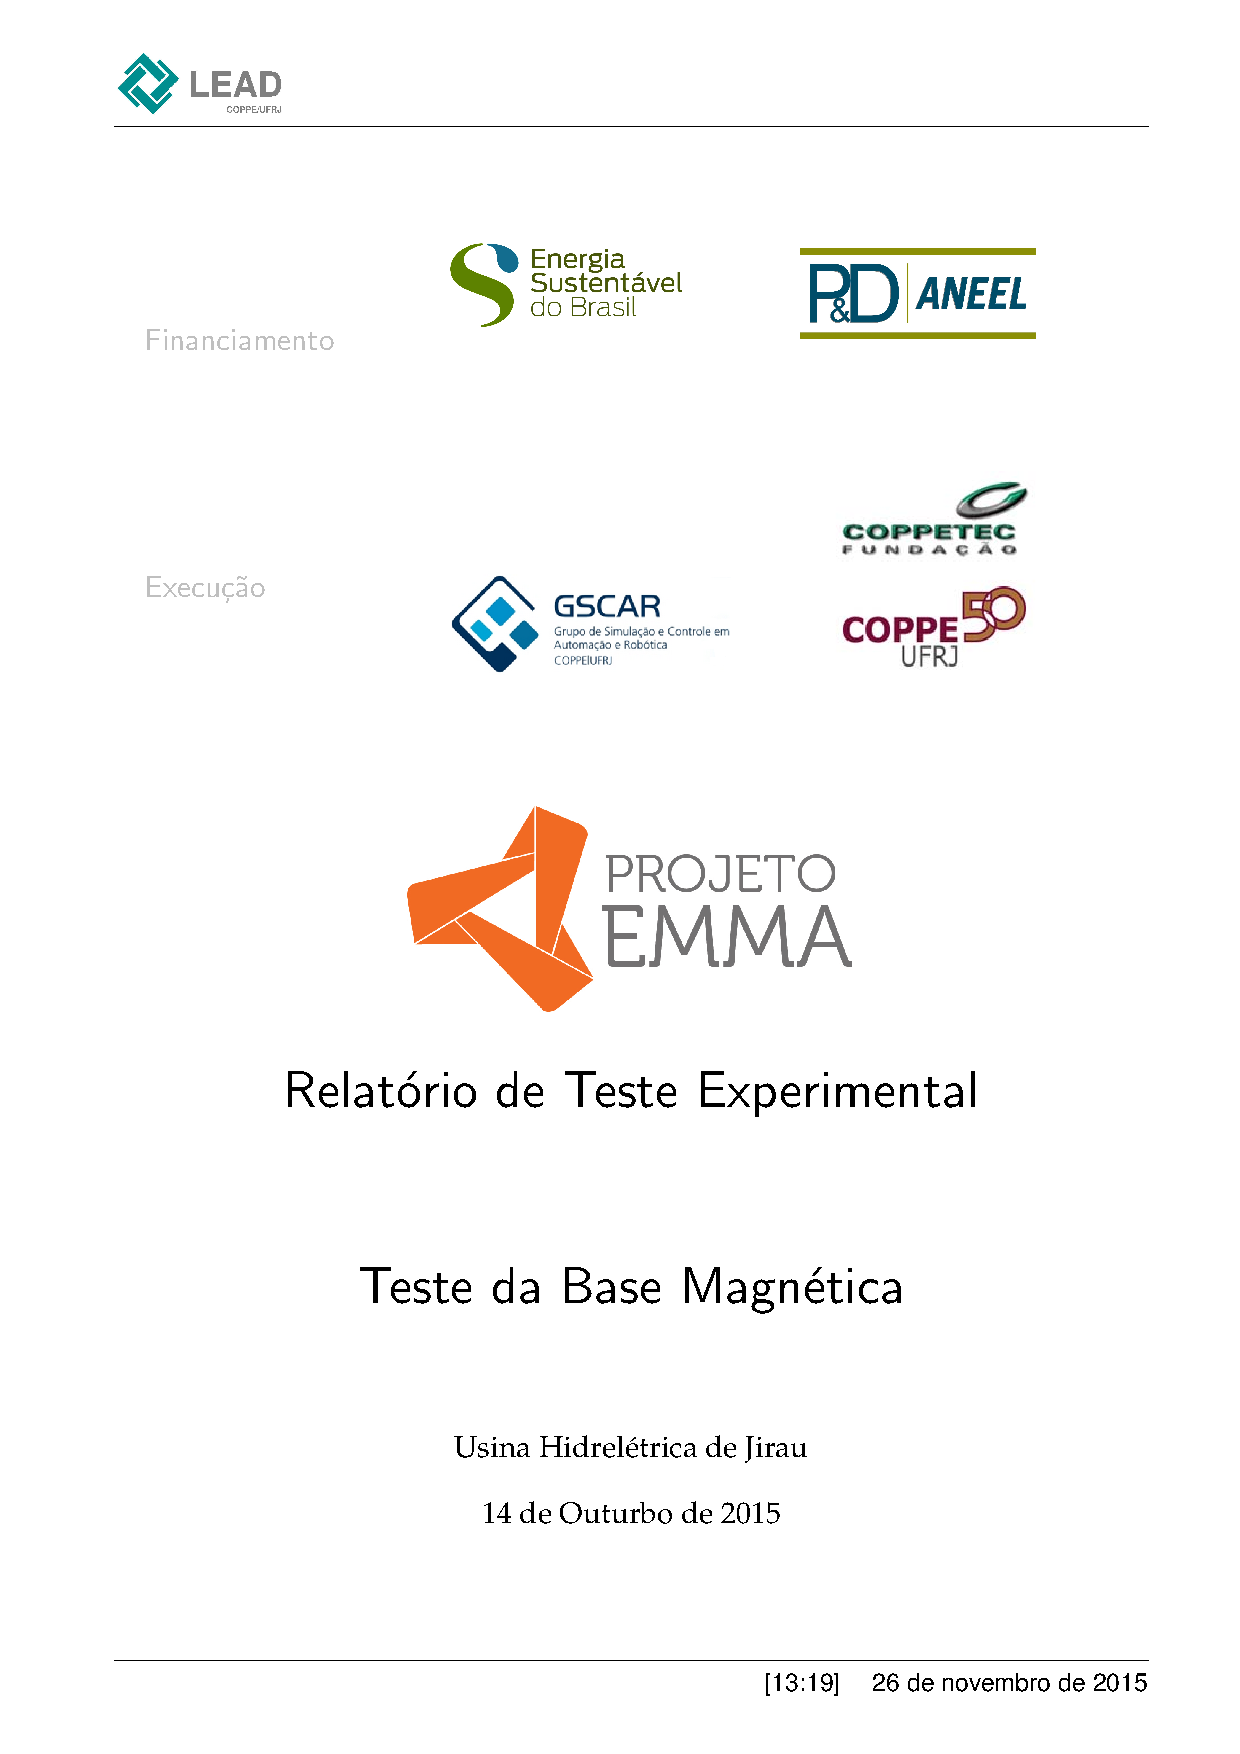
\includegraphics{Apendice/Relatorio_Teste_Base_Magnetica.pdf}
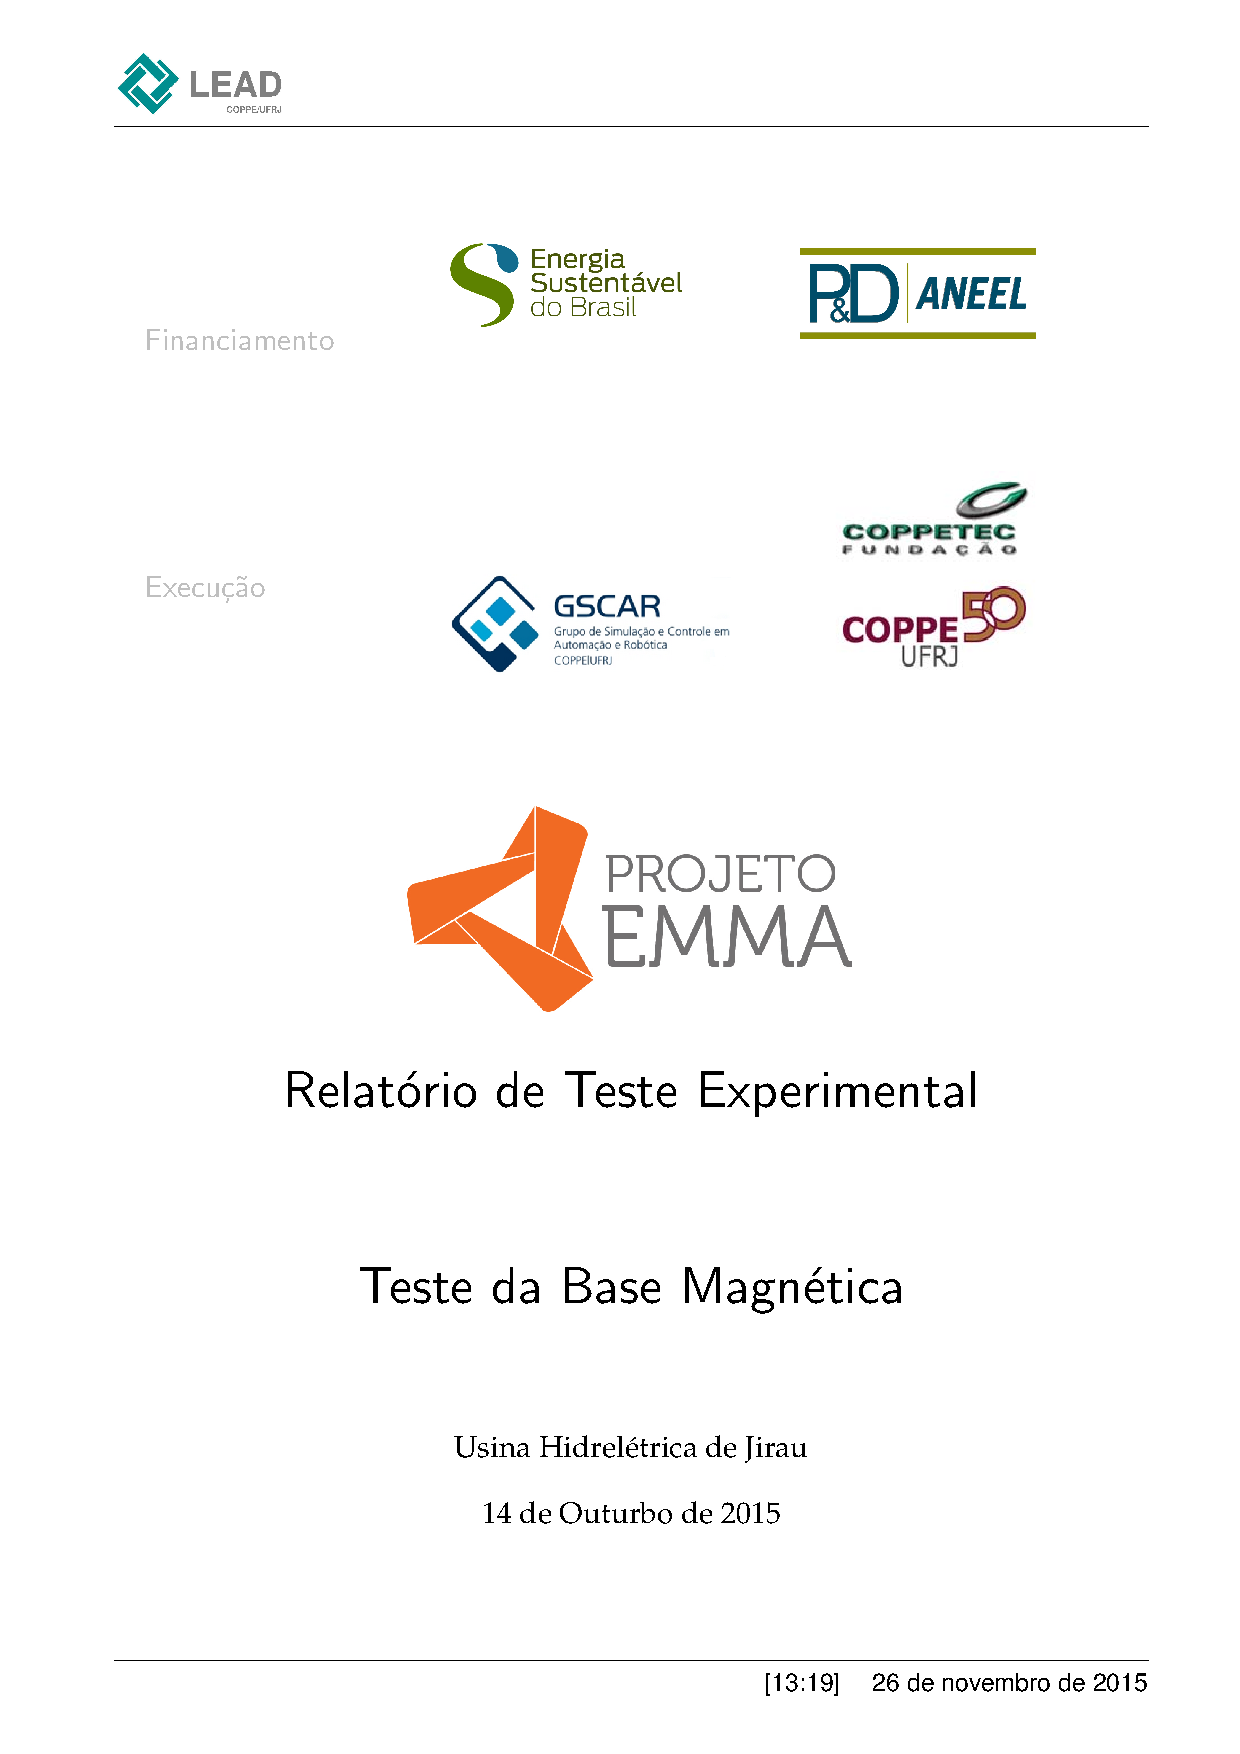
\includepdf[pages=1-,scale=0.9]{Apendice/Relatorio_Teste_Base_Magnetica.pdf}\label{ape::magnetic}
  
\bibliography{main} 
\appendix
\end{document}
